% !TeX program = xelatex
% !TeX encoding = UTF-8
\documentclass{MathModeling}
\usepackage{mwe,color,float}
\usepackage[linesnumbered,ruled]{algorithm2e}
\usepackage{setspace}
\usepackage{colortbl}
\usepackage[figuresright]{rotating}
\usepackage{rotating}
\usepackage{geometry}
\usepackage{graphics}
\usepackage{caption}
\usepackage{tablefootnote}
\everymath{\displaystyle}

\extrafloats{500}
\timu{\textbf{基于K-Means聚类与XGBoost的玻璃成分分析与鉴别}}
\keyword{可视化;XGBoost;K-means;斯皮尔曼相关性分析}
\begin{document}
\setcounter{page}{1}
\pagestyle{fancy}
	\begin{abstract}
		玻璃,我国丝绸之路早期贸易往来的宝贵物证。随着我国各地考古事业的推进,越来越多的玻璃文物被发现。值得注意的是,目前在预测玻璃文物风化前化学成分含量,玻璃文物的亚类划分,未知类型玻璃文物的归类及探究玻璃文物化学成分之间关联关系等问题的处理上,仍然存在一定的问题。
		本文将以{\textbf{铅钡和高钾两种玻璃文物}}为例,依据收集到的玻璃文物的基本信息,已分类及未分类玻璃文物的化学成分比例建立相关模型来解决上述问题。

		对于问题一,{\textbf{主要需要对数据进行预处理、以合适的方式探求与玻璃文物表面风化有关的因素、统计分析文物样品表面有无风化的化学成分统计规律及预测文物风化前的化学成分含量}}。由于数据存在{\heiti 多维、稀疏}的特征,我们选择将空缺行的数据删除以减少对后续问题求解的影响。
		{\heiti 对于子问题一},我们发现纹饰、颜色及玻璃类型为{\heiti 定类变量},我们选择使用{\textbf{卡方检验}}进行求解;
		{\heiti 对于子问题二},我们统计计算了风化前后各化学成分的均值,筛选出变化率较大的化学成分,并{\textbf{分类绘制箱线图}},对其风化前后化学成分含量的变化进行可视化分析,具体见\textcolor{blue}{\cref{高钾风化1}},\textcolor{blue}{\cref{高钾未风化1}},\textcolor{blue}{\cref{铅钡风化1}}及\textcolor{blue}{\cref{铅钡未风化1}}。
		{\heiti 对于子问题三},我们引入{\textbf{风化前后变化比}}的概念,对数据进行计算处理后,得出计算结果,具体结果见\textcolor{blue}{\cref{铅钡预测}}和\textcolor{blue}{\cref{高钾预测}}。

		对于问题二,{\textbf{主要需要依据文物化学成分给出文物类别划分依据并验证该分类依据的合理性及敏感性。}}
由于数据存在大量空缺,我们将空缺值视为{\heiti 该化学成分低于仪器可检测到的最低值,并将所有空缺值以0.04替代},减少对后续建模处理的影响。{\heiti 对于子问题一},我们首先筛选出高钾和铅钡玻璃风化前后的各化学成分比例,并绘制柱状体{\textbf{进行可视化处理}}以便分析,具体处理结果见\textcolor{blue}{\cref{高钾可视化}}和\textcolor{blue}{\cref{铅钡可视化}}。
{\heiti 对于子问题二},我们分析认为该问题属于{\textbf{数据的分类处理问题}},故我们采用K-means算法解决相关问题。为选定合理k值,我们使用{\textbf{肘部法则及可视化}}进行分析,具体处理结果见\textcolor{blue}{\cref{高钾亚类}}和\textcolor{blue}{\cref{铅钡亚类}}。

		对于问题三,{\textbf{主要需要对未知文物类型的玻璃文物进行分类并验证分类的合理性和敏感性}}。为合理解决该问题,我们{\textbf{建立了XGBoost模型}},
		将数据集划分为训练集和测试集,利用XGBoost算法得出了未知文物的分类结果,具体分类结果见\textcolor{blue}{\cref{分类结果}}。为验证该分类结果的敏感性,我们{\textbf{调整了部分化学成分的含量}},并再次对未知类型的玻璃文物进行分类处理,具体结果见\textcolor{blue}{\cref{调整后的分类结果}}。

		对于问题四,{\textbf{主要需要分析不同类别的玻璃文物中化学成分的关联关系及化学成分间的差异性}}。为合理探求各化学成分间的关系,我们选择采用{\textbf{斯皮尔曼相关性分析}}并绘制热力图进行分析,具体结果见\textcolor{blue}{\cref{高钾热力图}}和\textcolor{blue}{\cref{铅钡热力图}}。

		最后我们对所建立的模型进行合理性分析,同时对模型进行进一步推广。    
	\end{abstract}

	\section{问题的提出}
	\subsection{问题背景}
	玻璃,其在西亚和埃及地区往往被制作成珠形饰品,早期通过丝绸之路传入我国。为使玻璃在我国可以顺利生产,我国吸收其技术并将本土化改造,使之与外来玻璃制品外观相似而化学成分不同。
	
	玻璃的主要成分为二氧化硅,炼制时往往需要助熔剂,而助熔剂的不同往往会导致{\textbf{玻璃的成分比例不同}}。我们据此将玻璃分类,例如:铅钡玻璃({\textbf{铅矿石}}为助熔剂),钾玻璃({\textbf{草木灰等含钾量较高的物质}}为助熔剂)。示意图如\textcolor{blue}{\cref{玻璃制造示意}}所示。
	
	\begin{figure}[H]
		\centering
\includegraphics[width=0.6\textwidth]{图1.jpg}
		\caption{玻璃制造示意图}
		\label{玻璃制造示意}
	\end{figure}

	古代玻璃极易受埋藏环境的影响而风化,在此过程中{\textbf{玻璃的内部和外部元素会发生大量交换}},其成分比例会发生一定的变化,对玻璃类型的判别产生一定的干扰,故我们需要利用已有数据建立通用,可靠的模型以判断玻璃所属类别。

	
	\subsection{问题要求}
	\begin{itemize}
		\item \textbf{问题一}:(1)分析{\textbf{玻璃类型、纹饰和颜色}}与表面风化是否有关;(2)根据{\textbf{玻璃类型}},分析文物表面有无风化的统计规律;(3)根据{\textbf{风化点监测数据}}预测出玻璃在风化前的各化学成分含量。
		\item \textbf{问题二}:(1)根据{\textbf{表单1、2中的数据}}分析并得出玻璃的分类规律;(2){\textbf{依据分类规律}},使用合适的方法,在各类别选择恰当的化学成分进行亚类划分并展示结果;(3)分析上述结果的{\textbf{合理性和敏感性}}。
		\item \textbf{问题三}:(1)分析{\textbf{表单3}}中未知类别玻璃的化学成分并鉴别其所属类别; (2)分析结果的敏感性。
		\item \textbf{问题四}:(1)分析{\textbf{不同类别的玻璃文物样品}}化学成分之间的关联关系; (2)比较不同类别之间化学成分关联关系的差异性。
	\end{itemize}

	\section{问题的分析}
	\subsection{问题的整体分析}
	该问题是一个关于玻璃文物风化前后化学成分比例分析,建立判定玻璃文物类别模型的问题。
	
	\textbf{从分析目的看},本题需要在风化导致的化学成分比例偏移的情况下鉴别玻璃文物的类别。其中任务包括了:1、分析风化对不同类型的玻璃文物化学成分含量的影响,并能通过风化后成分预测风化前成分; 2、选择合适的化学成分对玻璃文物合理分类,确定分类标准; 3、选择位置类别的玻璃文物进行化学成分分析,检验分类模型的稳定性和包容性。

	\textbf{从数据来源、特征看},本题的数据来源于考古工作者。数据包括:玻璃文物的基本信息;已分类玻璃文物的化学成分比例;未分类玻璃文物的化学成分比例。这些数据具有多维,稀疏的特性且其成分比例累加和应为100$\%$。基于本题中数据的特征,应对数据进行一定的{\textbf{预处理}}。

	\textbf{从模型的选择看},本题的数据量较小,且需预测玻璃中的成分含量并对玻璃进行分类,因此本文并未采用过于复杂的模型,而是建立了{\heiti 风化后化学成分变化比}和{\heiti k-means聚类}两类模型。

	\textbf{从编程软件的选择看},本题为{\textbf{数据分析类}},需要将相关数据进行预处理、分析及可视化,并依据各设问建立不同类别的模型,因此我们选择基于{\textbf {Python 的 Jupyter Notebook}} 对问题进行求解,其交互式的编程方式较为轻量化,相较于其它软件更为方便高效。
	
	\subsection{问题一的分析}
	问题一的核心目的有以下几点:{\heiti 其一},{\textbf{对附件中的数据进预处理,剔除不符合要求的数据}};{\heiti 其二},{\textbf{分析并得出文物样品表面的有无分化化学成分含量统计规律}};{\heiti 其三},{\textbf{依据统计规律推算出玻璃文物风化前化学成分含量}}。对于已给定的数据集,数据在完整性方面存在着一定的缺陷,
	故不可由原始数据进行直接分析,须对数据进行预处理。我们选择直接剔除不符合要求的数据。此外我们发现{\heiti 玻璃类型、纹饰和颜色}均为定类数据,故采用卡方检验对表面风化与以上三者的关系进行研究。为了直观展现文物样品表面有无风化化学成分含量的统计规律,我们选择绘制两种玻璃有无风化时各化学成分占比的均值和各化学成分占比的箱线图。
	针对预测玻璃文物风化前化学成分含量这一问题,我们分析认为将附件中表单1与2的数据相互关联,建立风化前后化学成分变化比例模型以合理预测。

	\subsection{问题二的分析}
	问题二的核心目的在于{\textbf{根据文物的化学成分提出合理的文物分类的的依据并分析其合理性及敏感性}}。{\heiti 对于子问题一},我们选择对高钾和铅钡类型的玻璃数据绘制可视化图像,通过图像分析高钾、铅钡玻璃的分类规律;
	{\heiti 对于子问题二},我们分析采用{\textbf{K-means聚类分析}},通过肘部法则选择合适的k值,对高钾、铅钡玻璃进行亚分类。为了验证该模型是否足够稳定即{\heiti 验证风化文物原始成分的预测误差是否会造成明显的影响},我们微调了样本数据以测试其敏感性。

	\subsection{问题三的分析}
	问题三的核心目的在于{\textbf{利用未分类的玻璃文物以进一步验证分类模型的稳定性}}。我们分析选用{\textbf{XGboost模型}}以预测未知玻璃文物对应类型,通过轻微改变成分占比来测试分类模型的敏感性。


	\subsection{问题四的分析}
	对于该问题我们认为其核心目的在于{\textbf{在于以合理的方式提取数据中的有效特征}}。我们分析认为若需知晓两种类型的玻璃制品化学成分之间的关联关系,我们需要进行{\heiti 斯皮尔曼相关性分析}并画出热力图,同时结合两个玻璃类型之间化学成分的横向对比,最终得出其化学成分内部关联关系的差异性。
	
	\section{模型的假设}
	\begin{itemize}
		\item \textbf{假设一}:假设成分比例数据中的空缺值是由于成分含量过低且低于仪器所能检测到的含量下限造成并默认记为{\heiti 0.4}。
		\item \textbf{假设二}:假设各未分类玻璃文物的化学成分比例数据分别来自于各文物的某一采样点。
		\item \textbf{假设三}:假设所给化学成分数据的检测手段有效,结果准确无误。
		\item \textbf{假设四}:假设忽略颜色、纹饰、玻璃种类三者之间的内部影响。
	\end{itemize}
	\section{符号说明}
	\begin{center}
		\begin{tabularx}{0.7\textwidth}{c@{\hspace{1pc}}|@{\hspace{2pc}}X}
			\Xhline{0.08em}
			符号 & \multicolumn{1}{c}{符号说明}\\
			\Xhline{0.05em}
			$\chi^2$ & 卡方 \\
			$i$ & 自由度 \\
			$y$ & 因变量实际值\\
			$\hat{y}$ & 因变量预测值\\
			$L^{\left(t\right)}$ & 目标函数\\
			$r_s$ & 斯皮尔曼相关系数 \\
			\Xhline{0.08em}
		\end{tabularx}
	\end{center}

	\textbf{注:}这里并未列出其余变量,这是由于它们在不同小节处有不同的含义,同时该表中也未列出专有定义的变量,这些变量在使用时会在相应位置进行详细说明。

	\newpage 
	\section{模型的建立与求解}
	对于本题,本文模型的建立与求解部分主要分为数据的准备,模型的建立、求解、结果分析。\textcolor{blue}{\footnote{本文所有可视化图示均为矢量图,若读者在阅读时发现图示字体过小,可适当放大PDF页面,详细查看图示数据等。此外,本文所有图示、表格均已交叉引用,读者阅读PDF时可点击对应图表,进行跳转。}}
	\begin{itemize}
		\item \textbf{数据的准备}:	由题设可知,当成分比例累加和{\textbf{介于85$\%$$\sim$105$\%$}}之间的数据视为{\heiti 有效数据},分析附件二后我们发现第15号及第17号采样点玻璃文物的化学成分比例累加和均{\textbf{小于85$\%$}},显然为无效数据,应将其剔除。
		对于数据集中的空缺数据,我们认为是由于相关化学成分含量过低且低于仪器所能检测下限造成的,我们将所有的空缺数据以仪器检测含量下限0.04$\%$填充。
		\item \textbf{模型的建立、求解、结果分析}:对于给定的数据集,我们依据其特点建立合适的模型,研究并量化分析{\textbf{玻璃文物风化与其相关特征的关系;有无风化的化学成分比例的统计规律及玻璃文物的分类及亚类划分依据}}。
		同时还需要对位置类别的玻璃文物进行类别划分,并解释该划分方式的合理性和稳定性。最后依据不同类别的玻璃文物分析化学成分之间的关联关系及差异性。
	\end{itemize}
	\begin{figure}[H]
		\centering
		\includegraphics[width=0.5\textwidth]{图2_00.jpg}
		\caption{问题解决流程}
	\end{figure}
	\subsection{问题一模型的建立与求解}
	对于问题一,我们将其分为三个子问题进行求解。{\heiti 对于子问题一},分析表单数据,我们发现纹饰、玻璃类型、颜色、表面风化程度均为定类变量,因此我们选用卡方检验对其求解。即统计样本的实际观测值与理论推断值之间的偏离程度,
	实际观测值与理论推断值之间的偏离程度决定卡方值的大小。在进行卡方检验时需提出两个互为对立的假设:原假设和备择假设。原假设是我们想要推翻的假设,
	即:{\textbf{玻璃文物表面风化与玻璃类型,纹饰和颜色无关}},反之则为{\textbf{备择假设}}。我们通常先假设随机变量相互之间独立。然后通过观察样本数据来判断是否可以拒绝原假设,从而推断两个变量之间是否存在相关关系。其中皮尔逊卡方统计量,计算公式如下
	\begin{equation}
	\chi^2=\sum_{i=1}^{k}\frac{\left( f_i-np_i \right) ^2}{np_i}
	\end{equation}
	两者差异越大,卡方值越大,若P<a,则拒绝原假设,若P$\geq$a,则不拒绝原假设。(本题a=0.05)
	我们首先分别统计了纹饰,玻璃类型和颜色类别下风化和未风化的玻璃文物数量。
	其中纹饰类别下玻璃文物得到风化情况及相应计算结果如\textcolor{blue}{\cref{纹饰与风化}}所示;颜色类别下玻璃文物的风化情况及相应计算结果如\textcolor{blue}{\cref{颜色与风化}}所示;不同玻璃类型对应玻璃文物的风化情况及相应计算结果如\textcolor{blue}{\cref{玻璃类型与风化}}所示,	
	
	\begin{table}[hp]
		\centering
		\caption{纹饰类别下玻璃文物的风化情况}
		\begin{tabular}{ccc}
			\toprule
			\textbf{纹饰} & \multicolumn{1}{c}{\textbf{风化}} & \textbf{未风化} \\
			\midrule
			\textbf{A} & \multicolumn{1}{c}{11} & 11 \\
			\textbf{B} & \multicolumn{1}{c}{6} & 0 \\
			\textbf{C} & \multicolumn{1}{c}{17} & 13 \\
			\midrule
			\textbf{卡方计算值} & \multicolumn{2}{c}{4.9565} \\
			\midrule
			\textbf{P计算值} & \multicolumn{2}{c}{0.0839} \\
			\bottomrule
			\end{tabular}%		
		\label{纹饰与风化}%
	  \end{table}%
	\begin{table}[hp]
	    \centering	
		\caption{颜色类别下玻璃文物的风化情况及相关计算结果}
		\begin{tabular}{ccc}
			\toprule
			\textbf{颜色} & \multicolumn{1}{c}{\textbf{风化}} & \textbf{未风化} \\
			\midrule
			\textbf{黑} & \multicolumn{1}{c}{2} & 0 \\
			\textbf{蓝绿} & \multicolumn{1}{c}{9} & 6 \\
			\textbf{绿} & \multicolumn{1}{c}{0} & 7 \\
			\textbf{浅蓝} & \multicolumn{1}{c}{12} & 8 \\
			\textbf{浅绿} & \multicolumn{1}{c}{1} & 2 \\
			\textbf{深蓝} & \multicolumn{1}{c}{0} & 2 \\
			\textbf{深绿} & \multicolumn{1}{c}{4} & 3 \\
			\textbf{紫} & \multicolumn{1}{c}{2} & 2 \\
			\midrule
			\textbf{卡方计算值} & \multicolumn{2}{c}{6.2871} \\
			\midrule
			\textbf{P计算值} & \multicolumn{2}{c}{0.5066} \\
			\bottomrule
			\end{tabular}%		
		\label{颜色与风化}%
	  \end{table}%   	  
	  \begin{table}[htp]
		\centering
  		\caption{不同玻璃类型对应的玻璃文物风化情况及相应计算结果}
    	  \begin{tabular}{ccc}
			\toprule
			\textbf{玻璃类型} & \multicolumn{1}{c}{\textbf{风化}} & \textbf{未风化} \\
			\midrule
			\textbf{铅钡} & \multicolumn{1}{c}{28} & 12 \\
			\textbf{高钾} & \multicolumn{1}{c}{6} & 12 \\
			\midrule
			\textbf{卡方计算值} & \multicolumn{2}{c}{5.4518} \\
			\midrule
			\textbf{P计算值} & \multicolumn{2}{c}{0.0195} \\
			\bottomrule
			\end{tabular}		
  		\label{玻璃类型与风化}
	  \end{table}
	由于计算过程中涉及到自由度的计算,在此处补充自由度的计算方法:{\textbf{自由度=[行数-1]*[列数-1]}}。

	从卡方检验的结果可知,对于玻璃类型这一类别,P=0.0195,P小于a,有理由拒绝原假设,即认为是否风化与玻璃类型有关联性。而对于纹饰和颜色这两个变量,P分别为0.0839和0.5066,P均大于a,故没有理由拒绝原假设,即认为是否风化与纹饰和颜色均没有关联性。
	
	{\heiti 对于子问题二},我们首先将预处理过的数据按照玻璃类型分类计算风化前后各化学成分的平均值,由于数据量较大,具体结果详见附录图示部分中\textcolor{blue}{\cref{铅钡未风化}},\textcolor{blue}{\cref{铅钡风化}},\textcolor{blue}{\cref{高钾未风化}}和\textcolor{blue}{\cref{高钾风化}}。
	通过比较两组数据可知在所有化学成分中{\textbf{二氧化硅、氧化钾、氧化钙、氧化铝、氧化铁、五氧化二磷}}这五个化学成分的含量风化前后变化较大。为了使结果更直观,我们分别将组成两类玻璃的化学成分与各自对应的风化情况绘制为箱线图。
	
	其中高钾玻璃如\textcolor{blue}{\cref{高钾风化1}},\textcolor{blue}{\cref{高钾未风化1}}所示,
	\begin{figure}[htbp]
		\begin{minipage}[t]{0.5\textwidth}%并排放两张图片,每张占页面的0.5,下同。
			\centering
			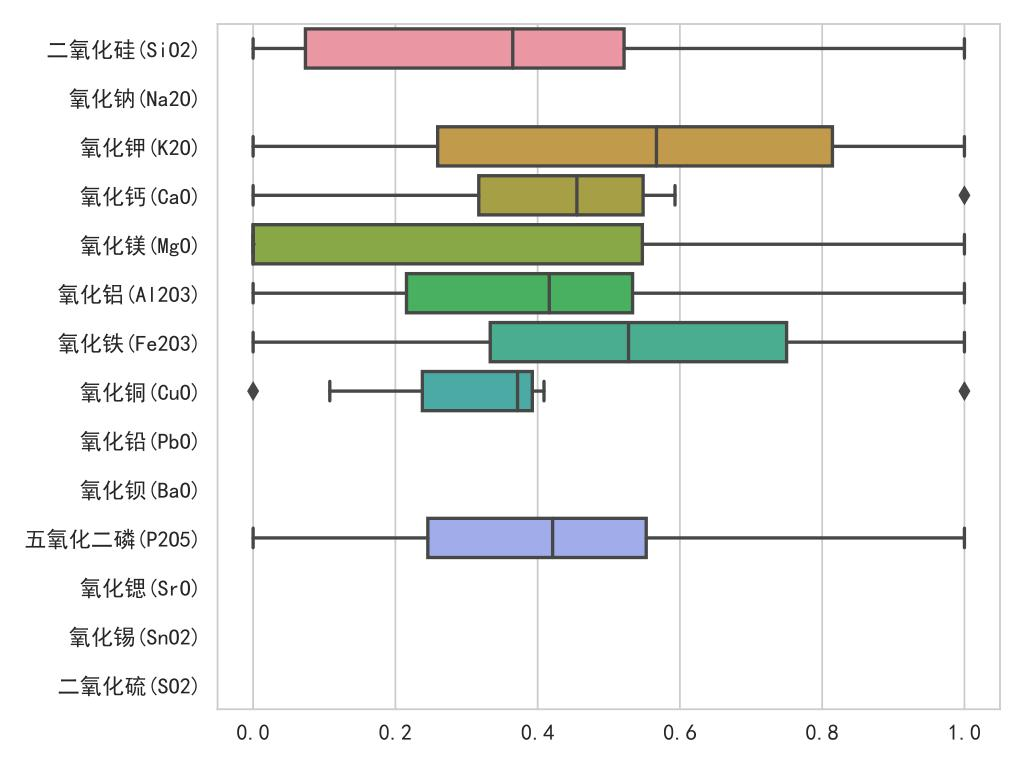
\includegraphics[width=\textwidth]{高钾风化箱线图_00.jpg}
			\caption{高钾风化箱线图.jpg}%注释1.jpg
			\label{高钾风化1}
			\end{minipage}
			\begin{minipage}[t]{0.5\textwidth}
			\centering
			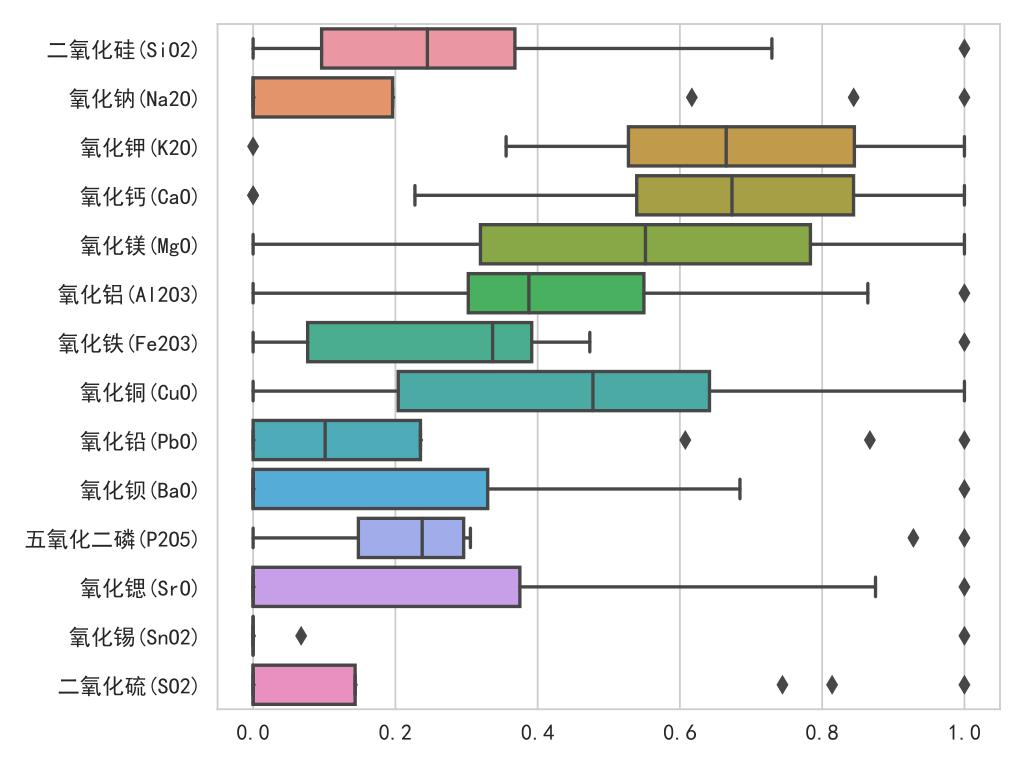
\includegraphics[width=\textwidth]{高钾未风化箱线图_00.jpg}
			\caption{高钾未风化箱线图.jpg}
			\label{高钾未风化1}
			\end{minipage}
			\end{figure}
	
		铅钡玻璃如\textcolor{blue}{\cref{铅钡风化1}}及\textcolor{blue}{\cref{铅钡未风化1}}所示,
	\begin{figure}[htbp]
		\begin{minipage}[t]{0.5\textwidth}%并排放两张图片,每张占页面的0.5,下同。
			\centering
			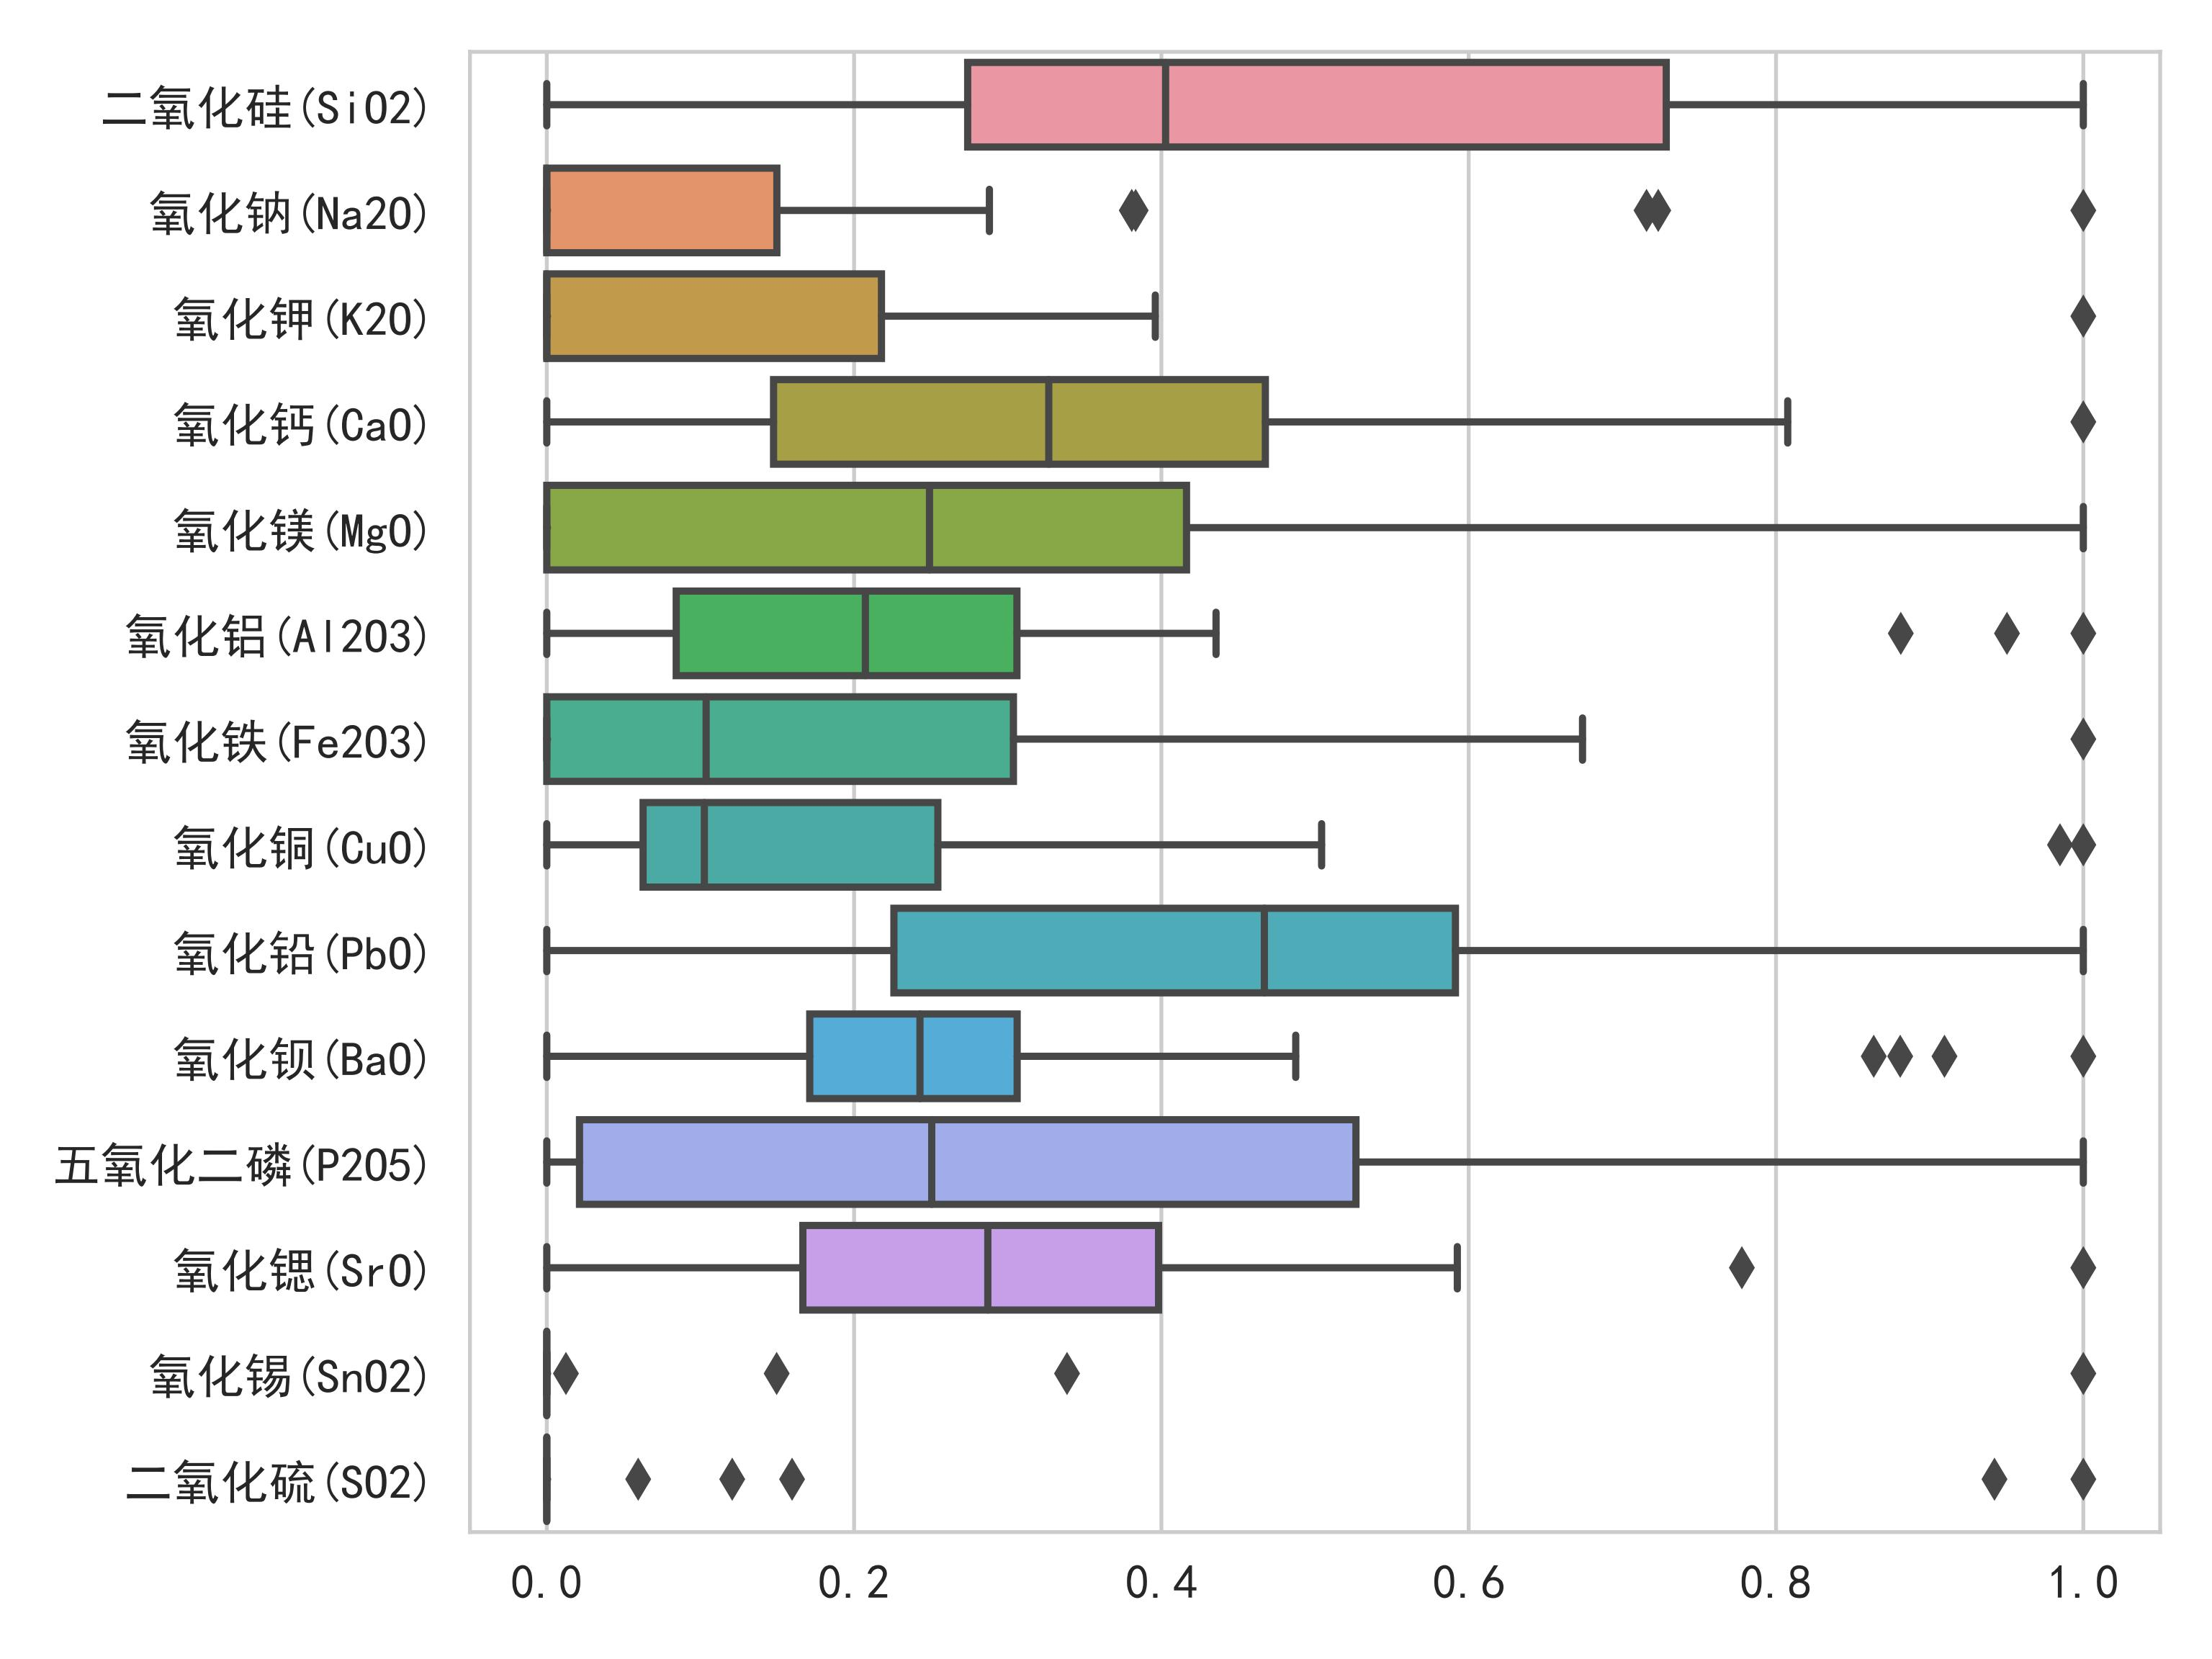
\includegraphics[width=\textwidth]{铅钡风化箱线图_00.jpg}
			\caption{铅钡风化箱线图}%注释1.jpg
			\label{铅钡风化1}
			\end{minipage}
			\begin{minipage}[t]{0.5\textwidth}
			\centering
			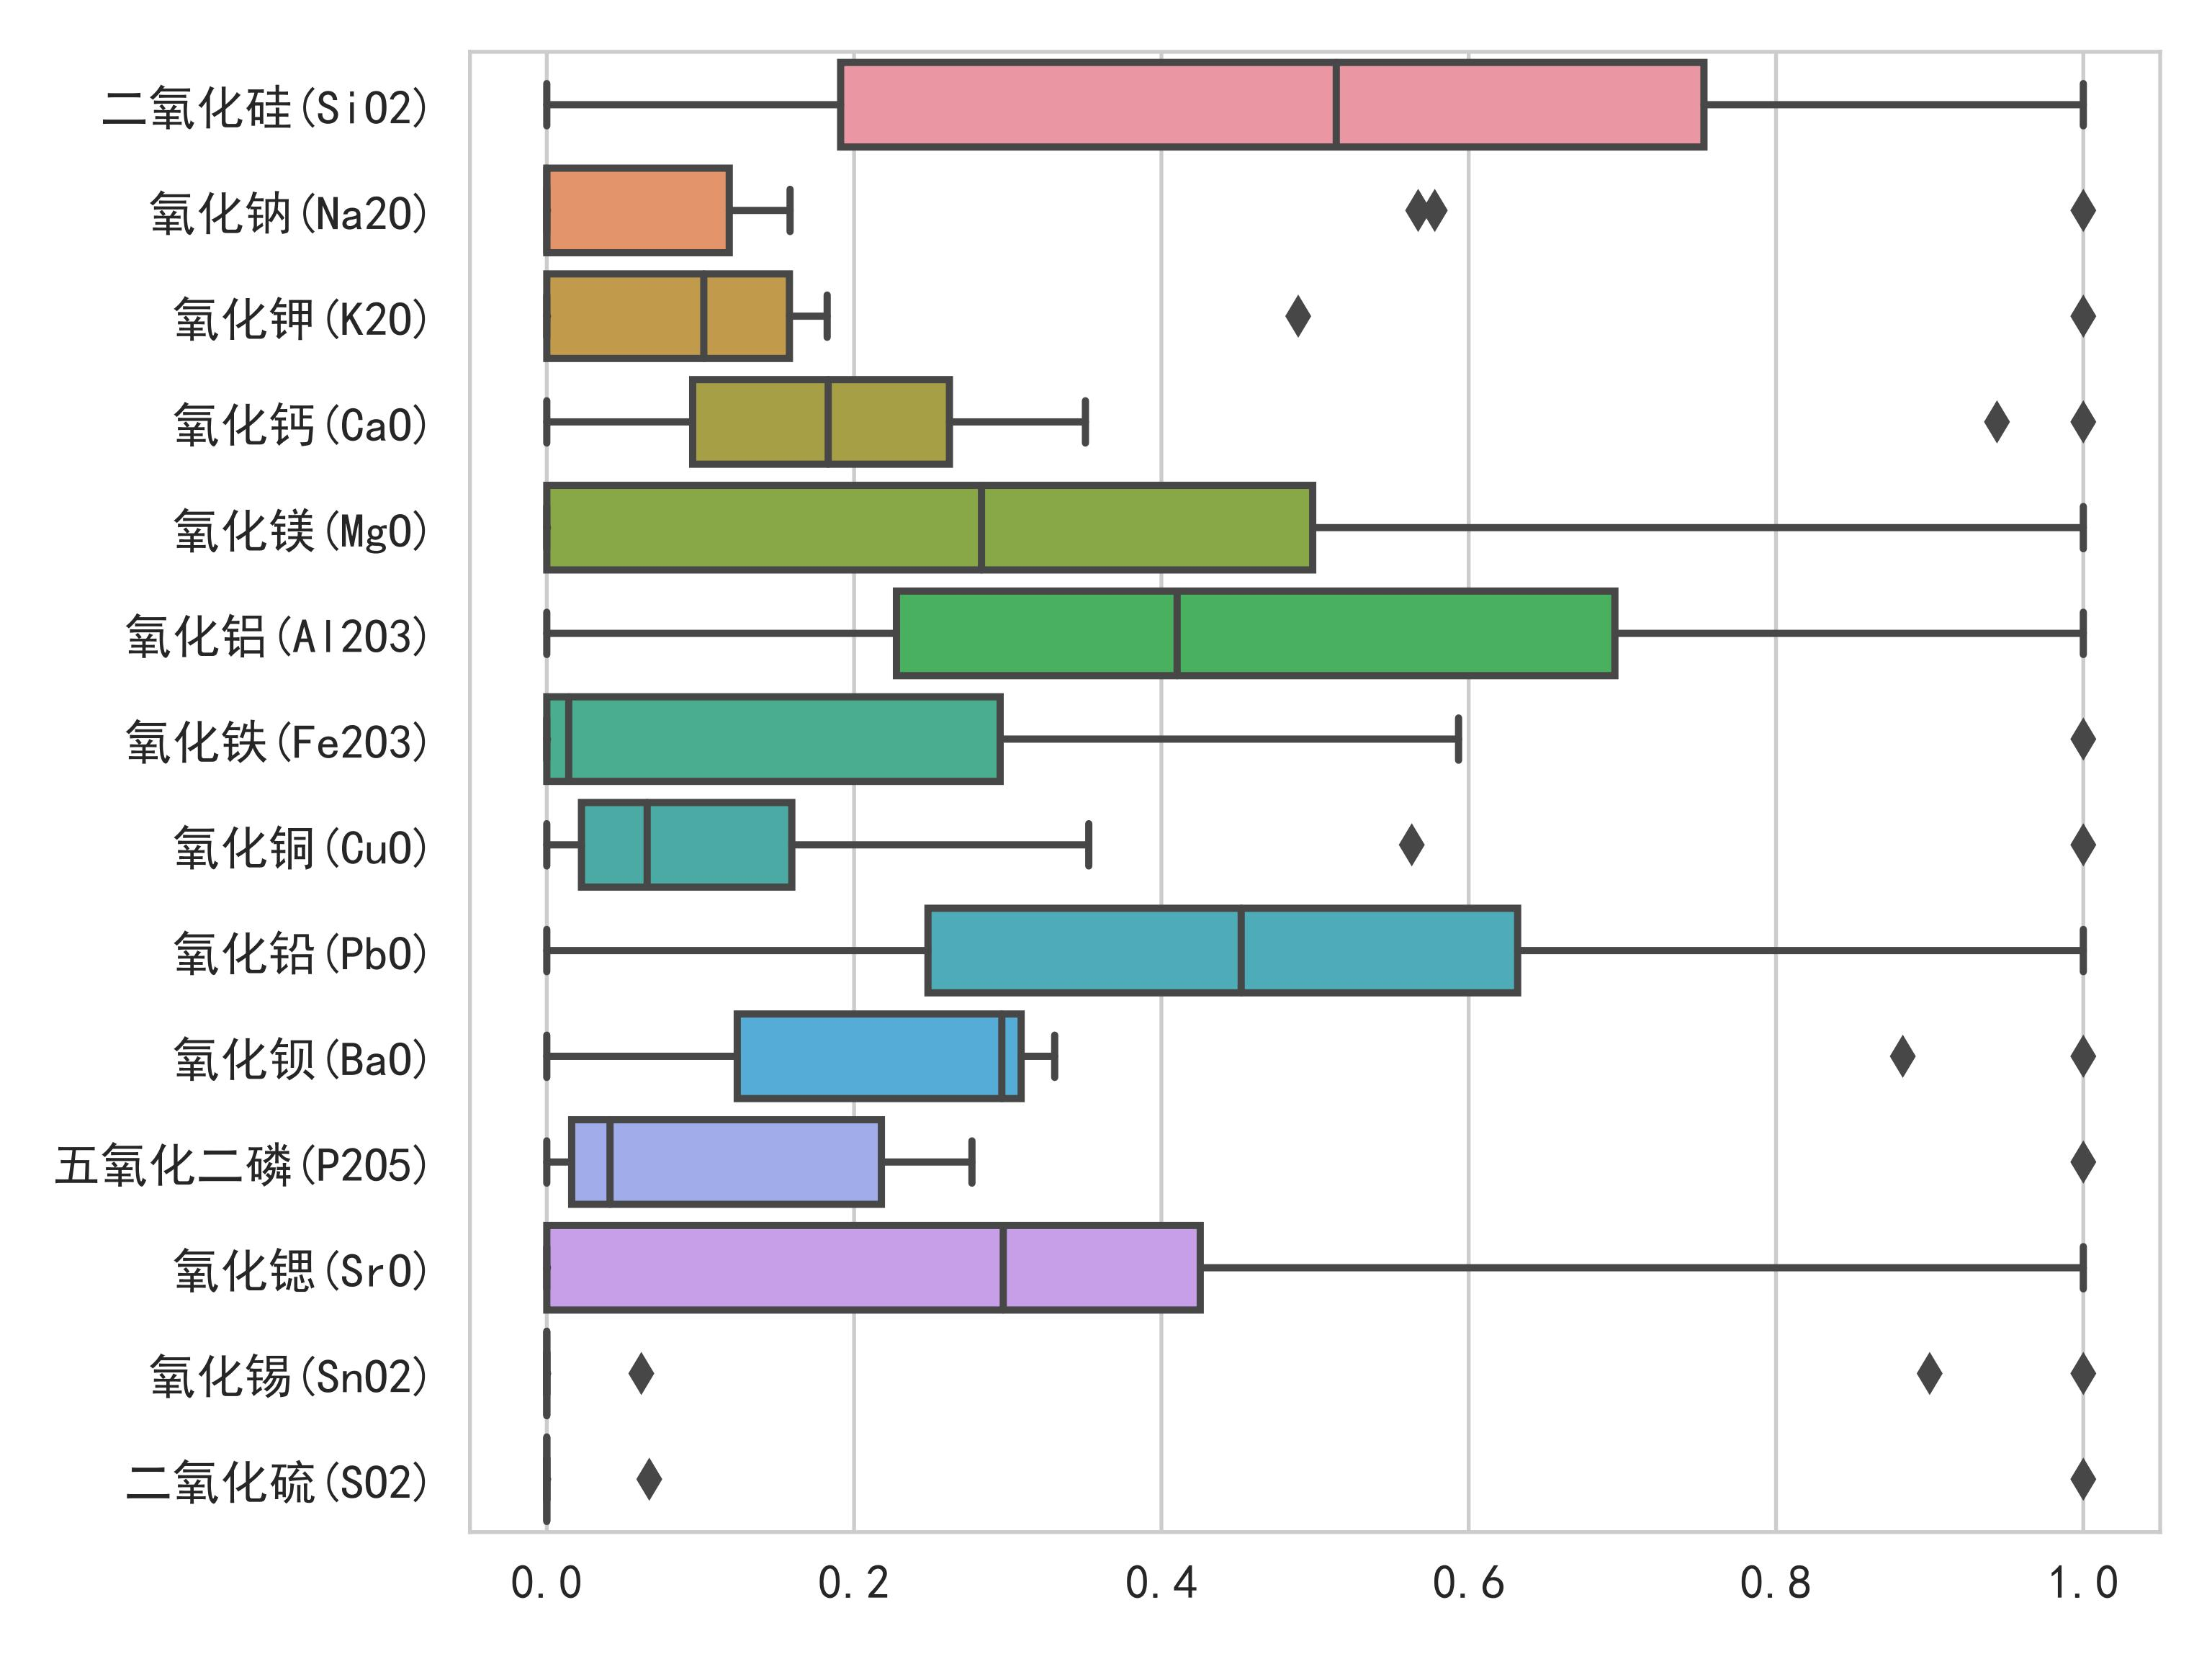
\includegraphics[width=\textwidth]{铅钡未风化箱线图_00.jpg}
			\caption{铅钡未风化箱线图}
			\label{铅钡未风化1}
			\end{minipage}
			\end{figure}
	
		通过观察比较上图,我们发现对于{\heiti 高钾玻璃},在风化后{\textbf{二氧化硅、氧化铁和五氧化二磷}}的含量明显上升,而{\textbf{氧化铜、氧化镁和氧化钙}}的含量明显下降。而{\heiti 铅钡玻璃},在风化后{\textbf{五氧化二磷、氧化铜和氧化钙}}的含量小幅上升,而{\textbf{氧化硅和氧化铝}}的含量小幅降低。
		此外,我们发现高钾类型的玻璃{\textbf{在风化后其主要化学成分呈下降趋势}},铅钡类型的玻璃{\textbf{在风化后其主要化学成分呈上升趋势}}。
	
		{\heiti 对于子问题三},我们通过附件可知每块玻璃文物由二氧化硅等共14个化学成分组成,我们设风化前某类型玻璃的某化学成分为${a_i}$,其中(i=1,2……14),风化后其含量为${b_i}$。
		则风化前某类型玻璃的某化学成分的占比我们设为${A_i}$,同理风化后其含量占比记为${B_i}$。为合理预测风化前化学成分含量,我们引入风化前后变化比${M_i}$的概念。风化前后变化比由分化前后的占比计算得出,具体公式如下
		\begin{equation}
		M_i=\frac{A_i-B_i}{B_i}
		\end{equation}
		   
		其中${A_i}$和${B_i}$的计算公式分别为$\frac{a_i}{\underset{i=1}{\overset{14}{\varSigma}}a_i}$,$\frac{b_i}{\underset{i=1}{\overset{14}{\varSigma}}b_i}$。
	
		经计算,铅钡玻璃(\textcolor{blue}{\cref{铅钡预测}})和高钾玻璃(\textcolor{blue}{\cref{高钾预测}})的预测结果如下,
	
	\begin{figure}[H]
		\centering
		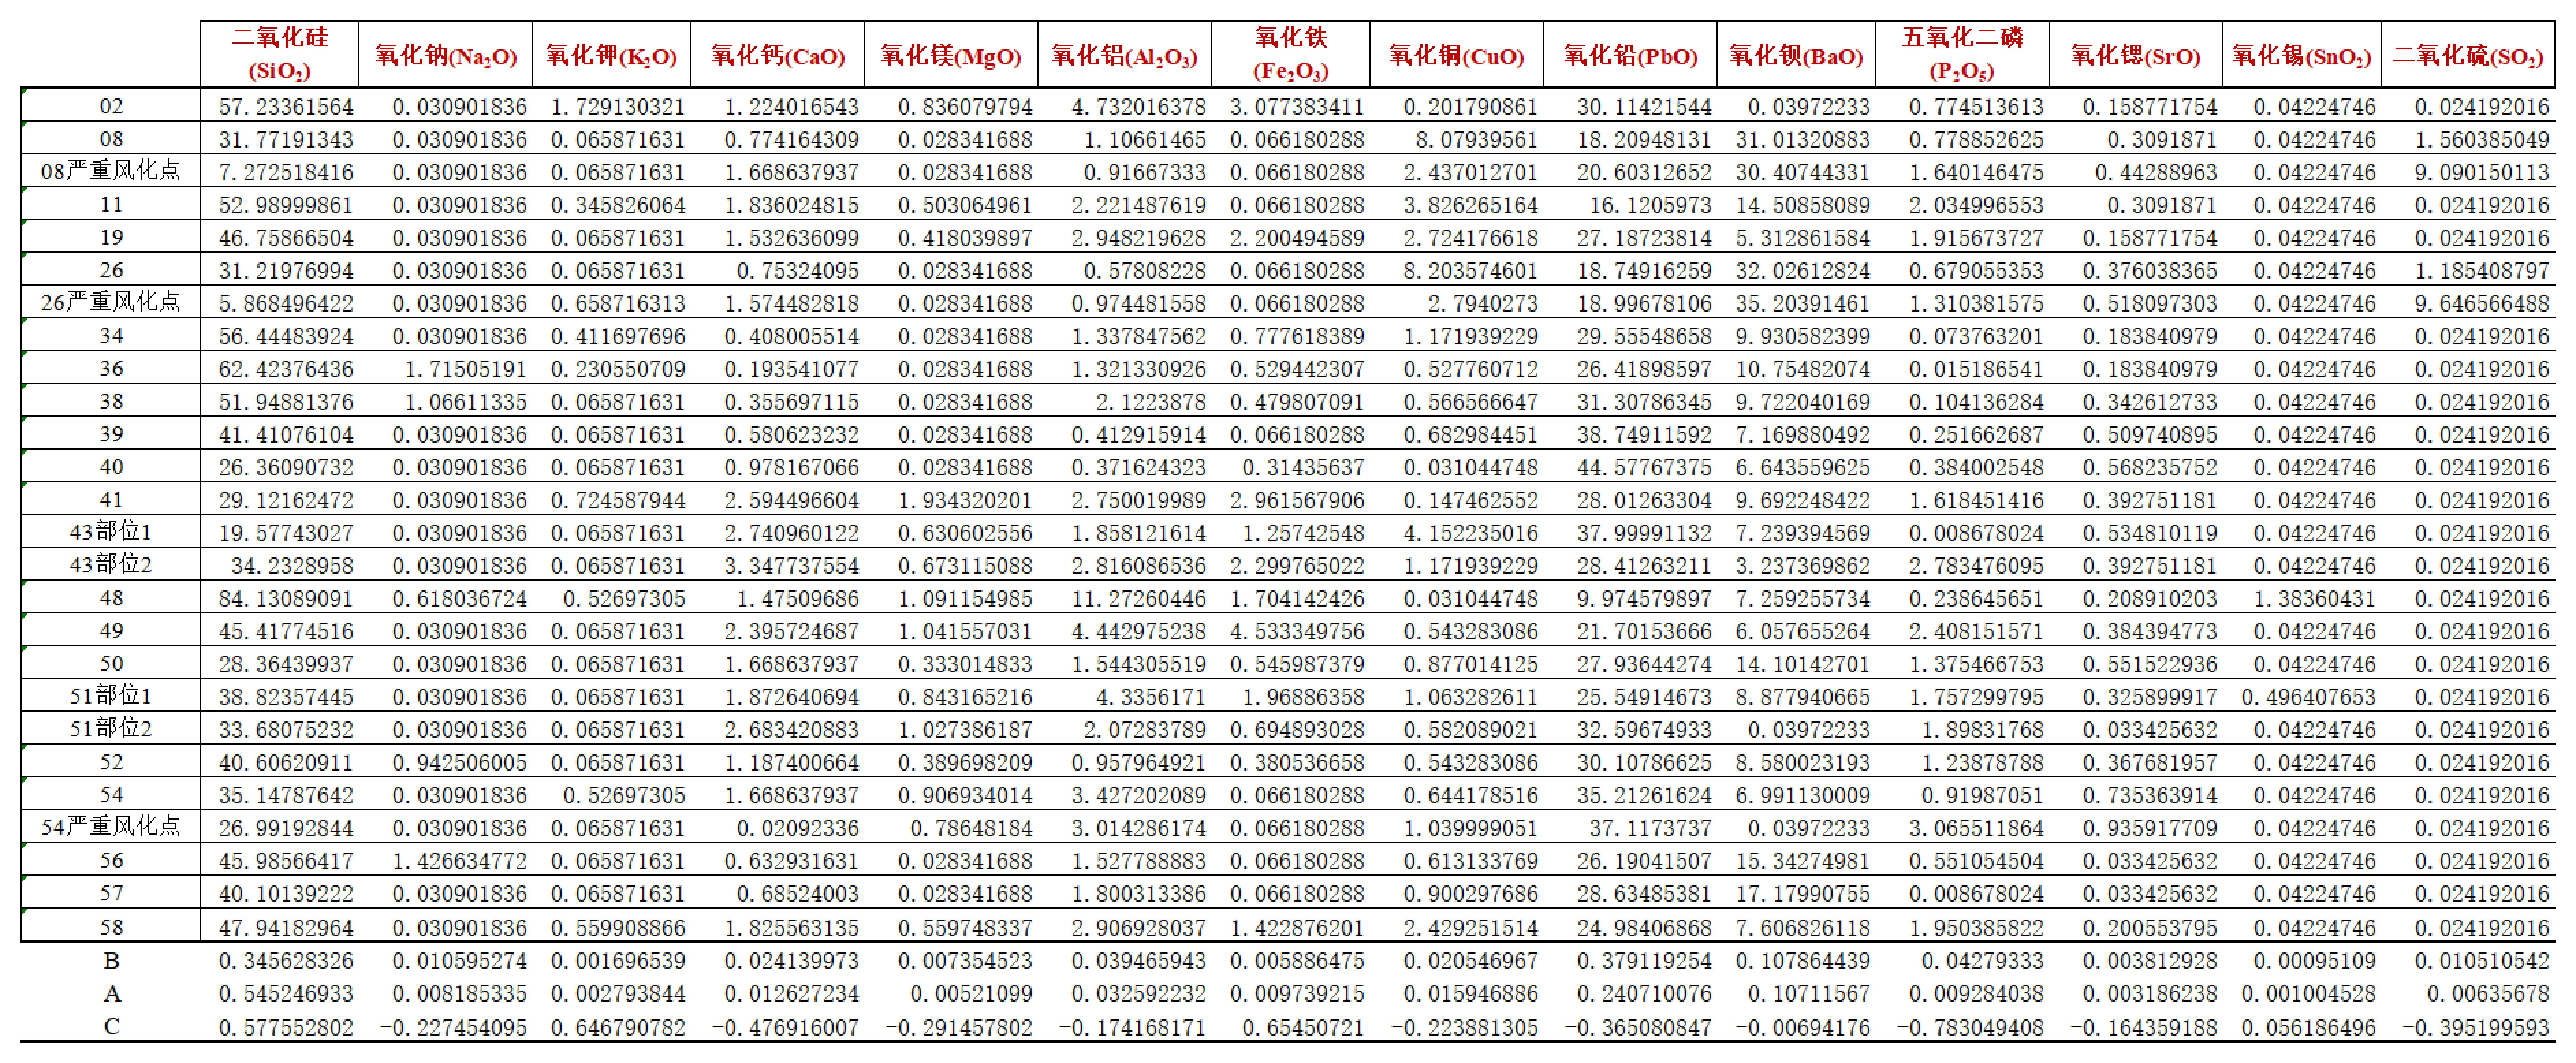
\includegraphics[width=0.7\textwidth]{铅钡预测_00.jpg}
		\caption{铅钡玻璃预测结果}
		\label{铅钡预测}
	\end{figure}
	\begin{figure}[H]
		\centering
		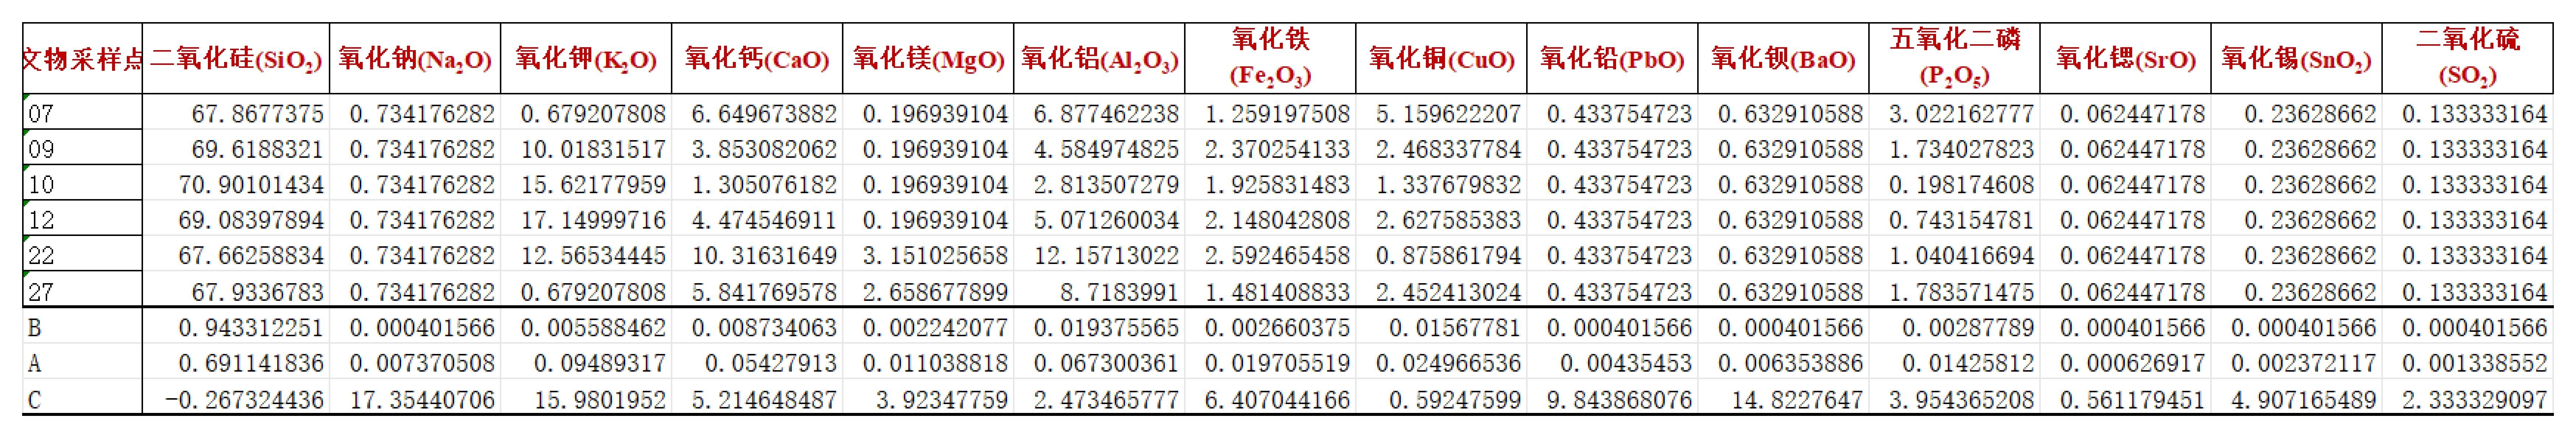
\includegraphics[width=1.0\textwidth]{高钾预测_00.jpg}
		\caption{高钾玻璃预测结果}
		\label{高钾预测}
	\end{figure}
 
	\subsection{问题二模型的建立与求解}
	对于问题二,我们将其分为两个子问题进行求解。

	{\heiti 对于子问题一},为分析出高钾和铅钡玻璃的分类规律,我们首先筛选出高钾和铅钡玻璃风化前后各化学成分的占比,并对筛选出的数据进行可视化处理。如\textcolor{blue}{\cref{高钾可视化}}和\textcolor{blue}{\cref{铅钡可视化}}所示。
	\begin{figure}[htbp]
		\begin{minipage}[t]{0.5\textwidth}%并排放两张图片,每张占页面的0.5,下同。
			\centering
			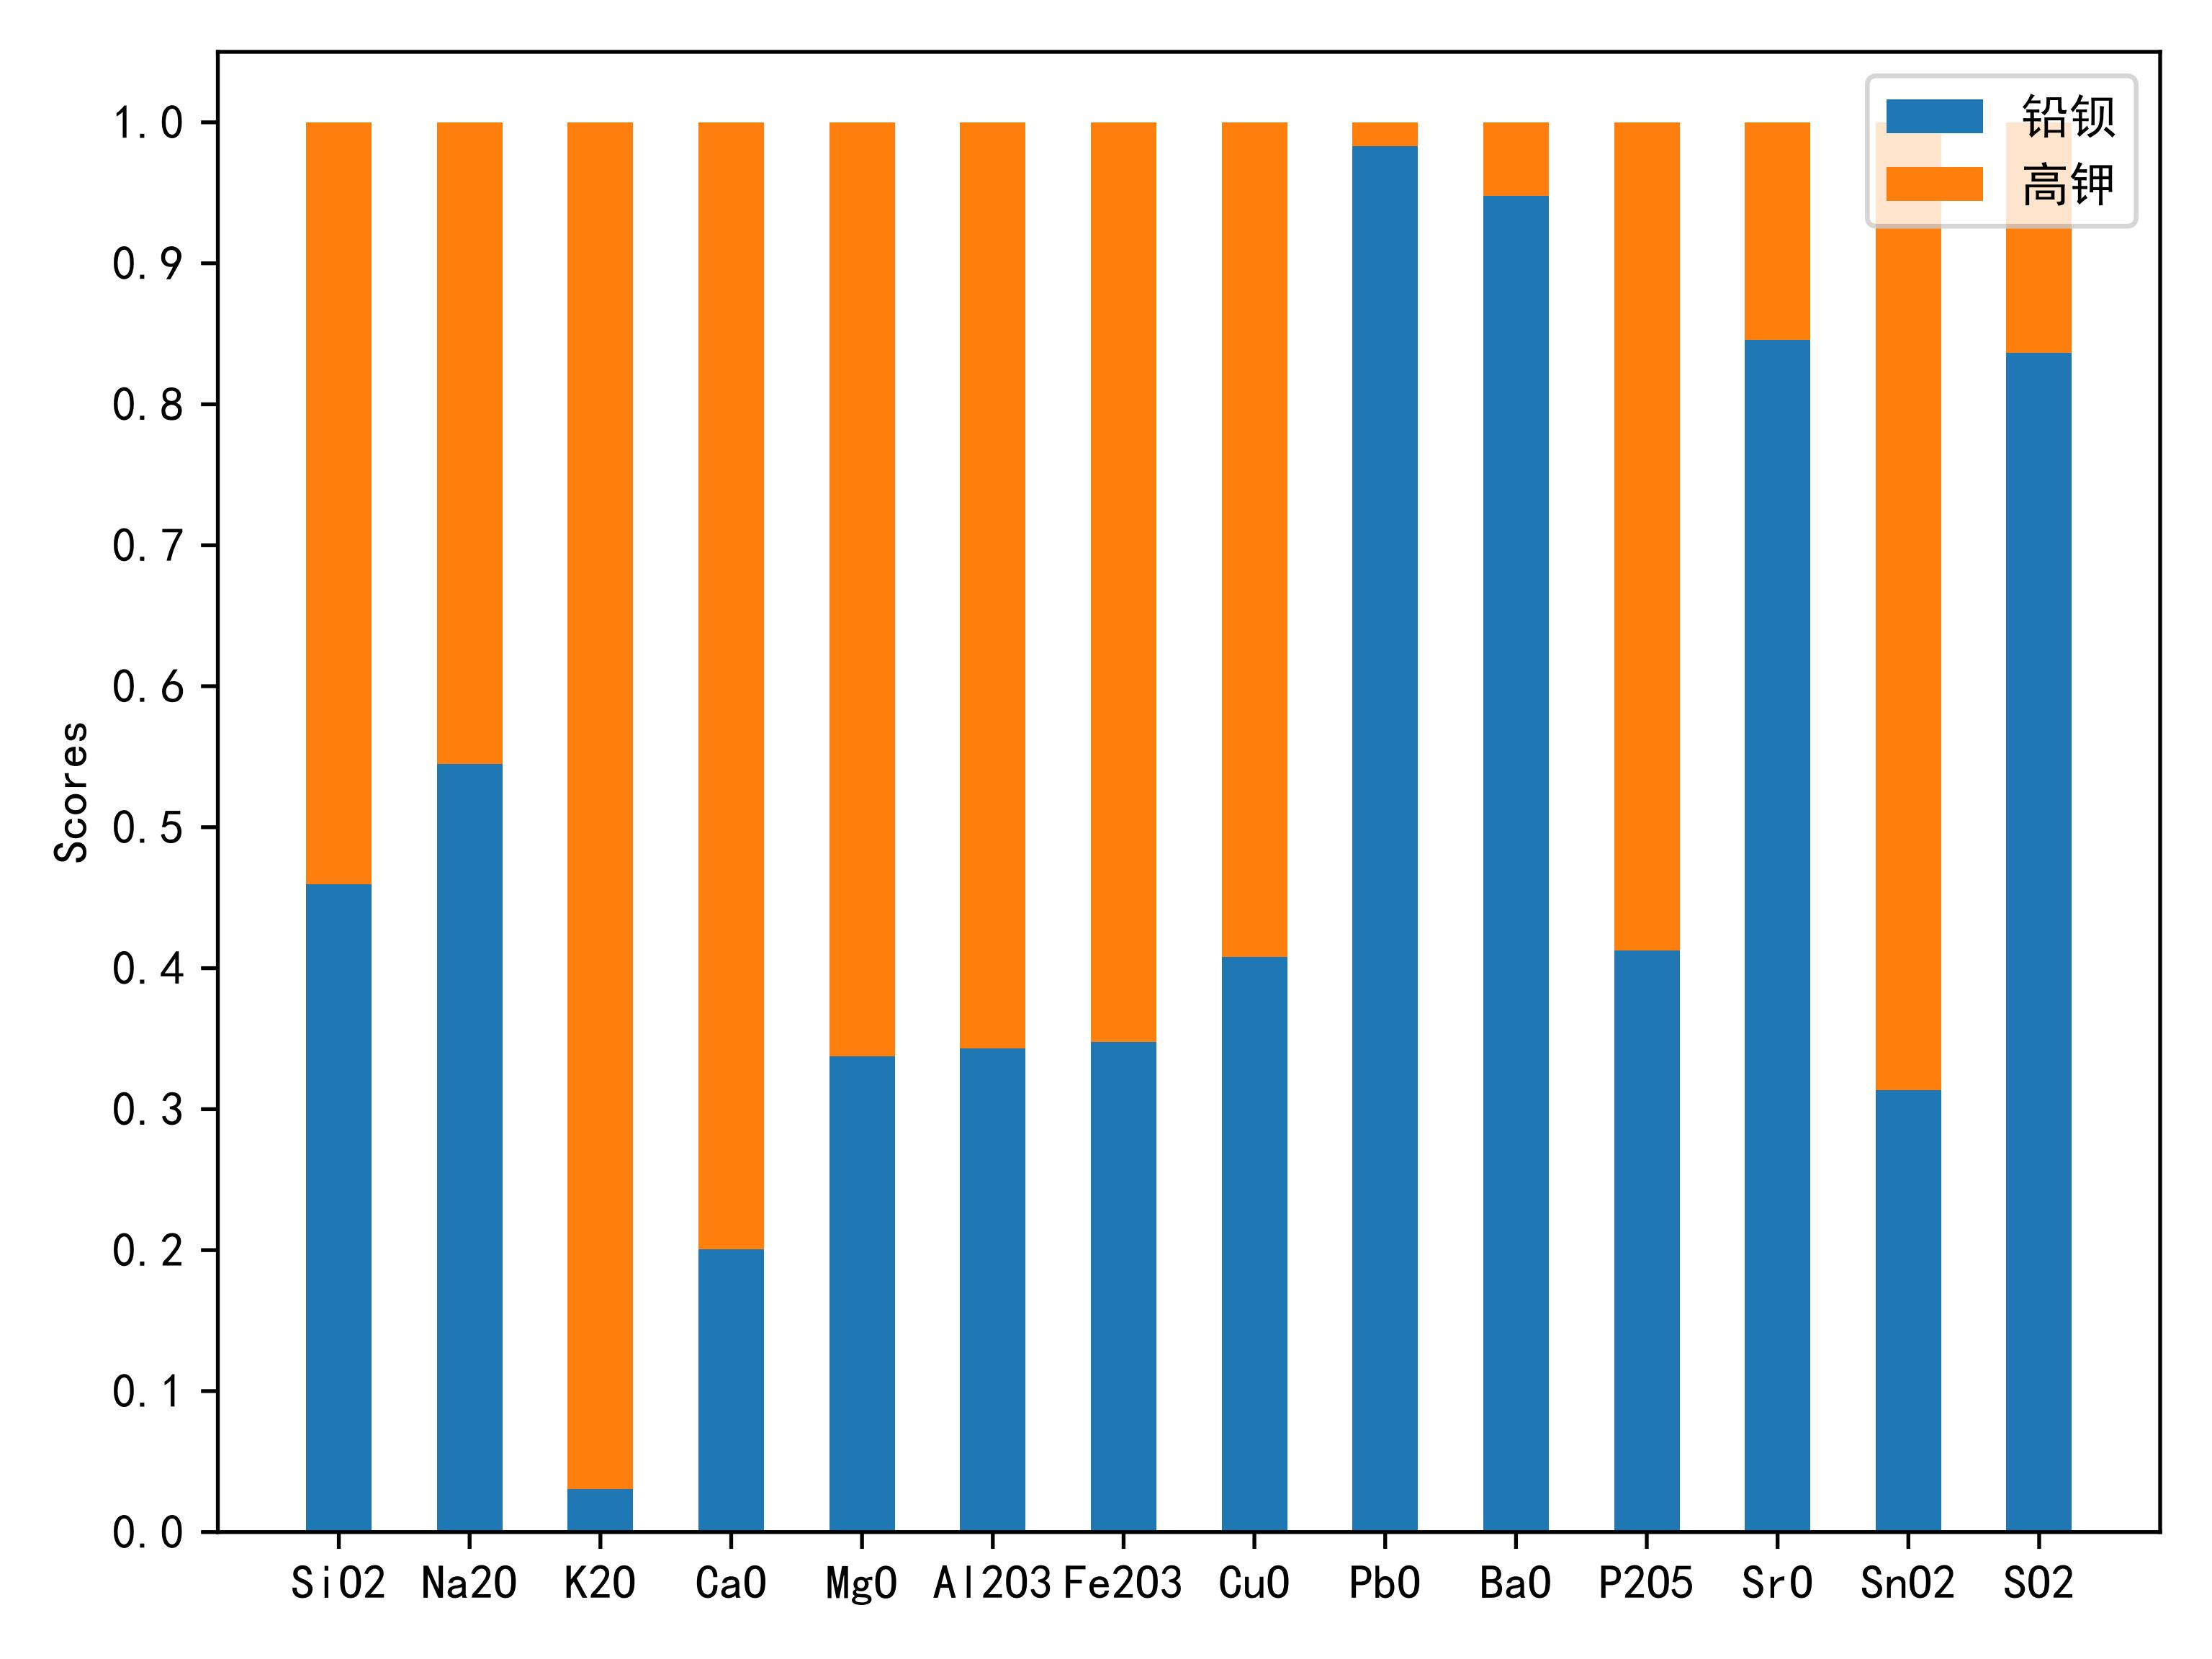
\includegraphics[width=\textwidth]{高钾问题二第一问_00.jpg}
			\caption{高钾玻璃风化前后各化学成分的占比}%注释1.jpg
			\label{高钾可视化}
			\end{minipage}
			\begin{minipage}[t]{0.5\textwidth}
			\centering
			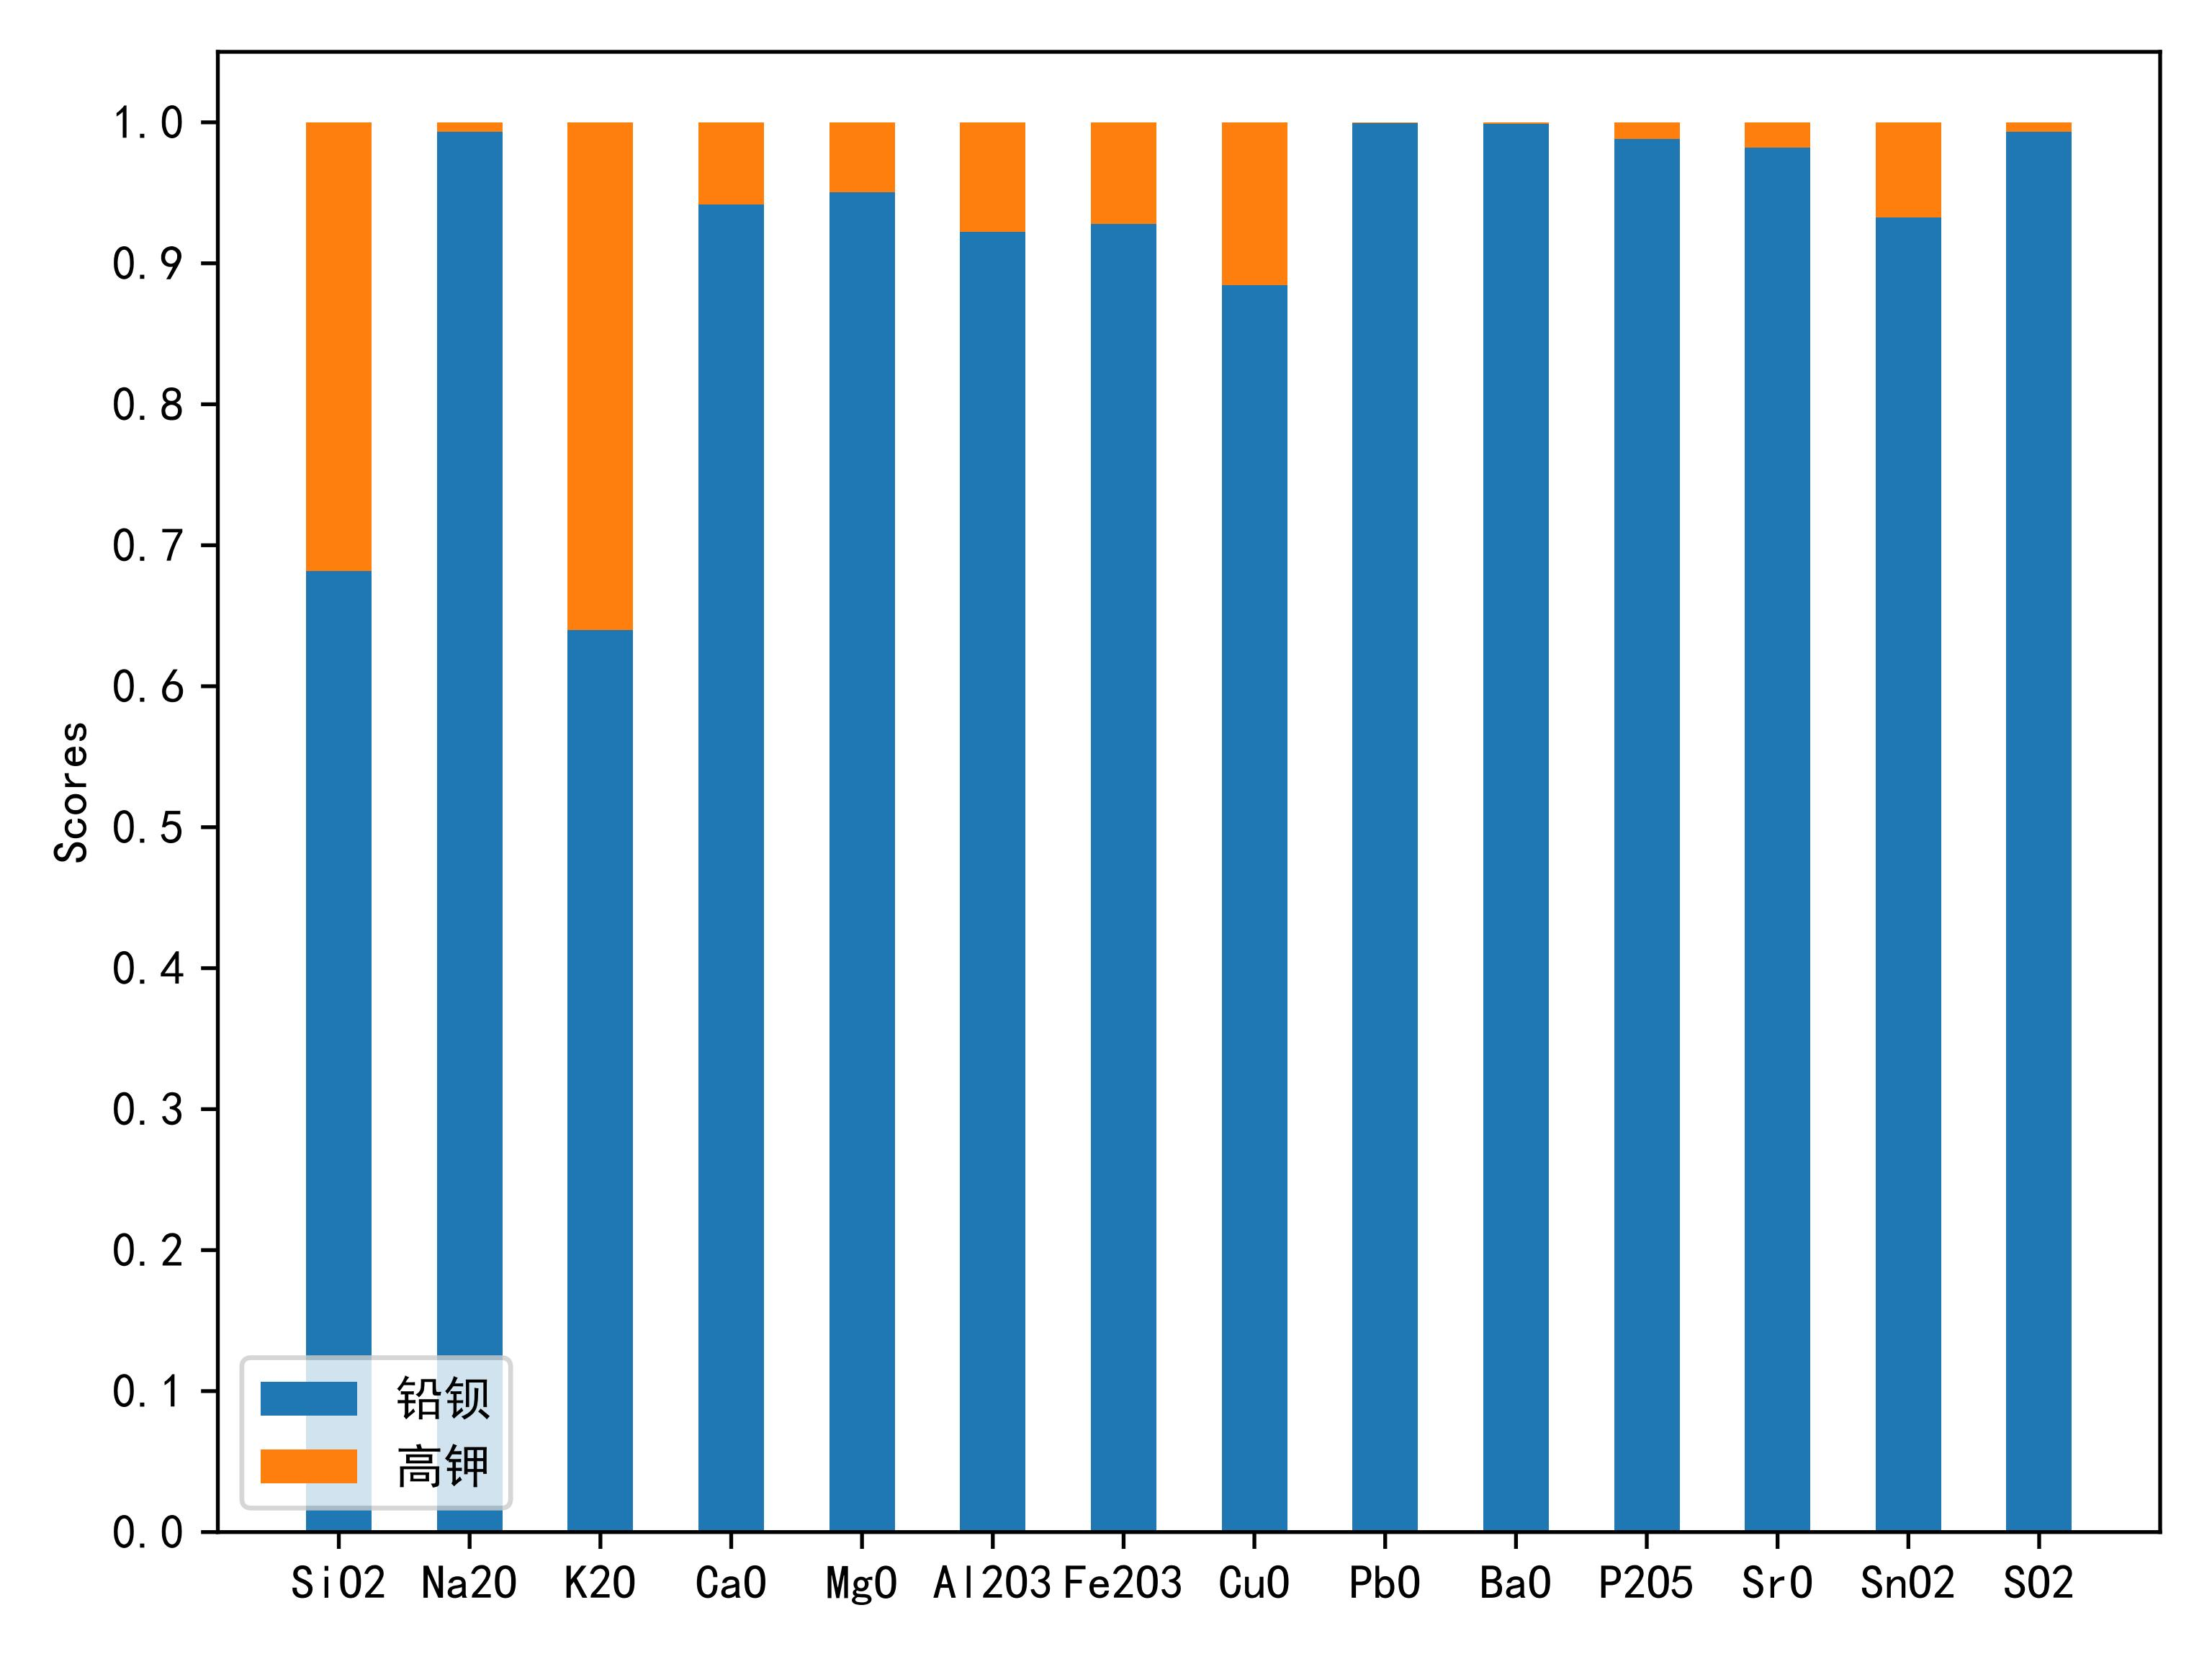
\includegraphics[width=\textwidth]{铅钡问题二第一问_00.jpg}
			\caption{铅钡玻璃风化前后各化学成分的占比}
			\label{铅钡可视化}
			\end{minipage}
			\end{figure}
	
	观察柱状图,我们发现高钾玻璃中{\textbf{氧化铅与氧化钡}}的含量远低于铅钡玻璃而其{\textbf{氧化钾}}的含量远超铅钡玻璃。

	由以上分析可知,{\heiti 高钾玻璃}相较于铅钡玻璃而言含有{\heiti 更多的氧化钾},但其氧化铅和氧化钡的含量远没有铅钡玻璃高。{\heiti 此结果与题目所说铅钡玻璃在烧制过程中加入铅矿石作为助熔剂,高钾玻璃的助熔剂是含钾较多的草木灰一致}。

	{\heiti 对于子问题二},题目要求对各类别选择合适的化学成分对玻璃文物进行亚类划分,为数据的分类处理的问题,而{\textbf{聚类分析}}的方法在处理这类问题时起到重要的作用。需要注意的是,{\heiti 聚类算法}属于无监督算法,其可通过样本的相似度将样本分为若干类,使得同一类内部的样本相似度尽可能高,不同类别之间的样本相似度尽可能低。
	本题我们采用{\textbf{k-means算法}}进行亚类划分,为了简化模型,我们剔除了含量过高和过低的数据和一些很难作为聚类依据的均匀数据。

	使用{\textbf{k-means算法}},其目的是将目标数据点分成类簇,找到每个簇的中心并使其度量最小化。过程为将数据集聚集成$k$个类簇,从数据集中随机选择N个数据点作为数据中心,分别计算出每个点到每个数据中心的距离,并将每个点划分到离其最近
	数据中心的类簇,在数据中心聚集了一些点后,重复上述过程,选出新的数据中心,比较第一次和第二次得到的数据中心。若两个数据中心之间的距离小于某一临界值,则此聚类达到了期望,算法终止;若距离相差很大,则继续执行算法,直到算法终止。
	
	K-means 算法{\heiti 首先}需要从给定的数据对象中随机指定初始聚类数$k$和相应的初始聚类中心C。然后计算从初始聚类中心到其余数据对象的距离。本文选择欧氏距离进行计算。从聚类中心到空间中其他数据对象的欧氏距离公式为
	\begin{equation}
		d\left( x,C_i \right) =\sqrt{\underset{j=1}{\overset{m}{\varSigma}}\left( x_j-C_{ij} \right) ^2}
	\end{equation}
	其中$x$为数据对象,$C_i$是第$i$个距离中心,$m$为数据对象的维度,$x_j$为数据$x$的第$j$个维度与聚类中心$C_i$的属性值。

	根据欧氏距离,测量相似度,并将与聚类中心相似度最高的目标数据分配到$C_i$类别。同类化之后,对$k$个聚类中的数据对象进行平均计算,形成新一轮的聚类中心,从而降低数据集的{\textbf{误差平方和(Sum of Square Error,SSE)}},其计算公式如下
	\begin{equation}
		\mathrm{SSE}=\sum_{i=1}^{k}\sum_{x\epsilon C_i}\left| d\left( x,C_i \right) \right|^2
	\end{equation}
	{\textbf{SSE}}被用来衡量聚类结果的效果。当其不再变化或收敛时,即停止迭代,得到最终结果。

	为了更好地对玻璃类型进行亚类划分聚类,我们需要确定合适的$k$值,因此我们使用肘部法则,绘制肘部法则可视化,确定最适$k$值,如\textcolor{blue}{\cref{铅钡肘部法则}}和\textcolor{blue}{\cref{高钾肘部法则}}所示。
	
		\begin{figure}[htbp]
			\begin{minipage}[t]{0.5\textwidth}%并排放两张图片,每张占页面的0.5,下同。
			\centering
			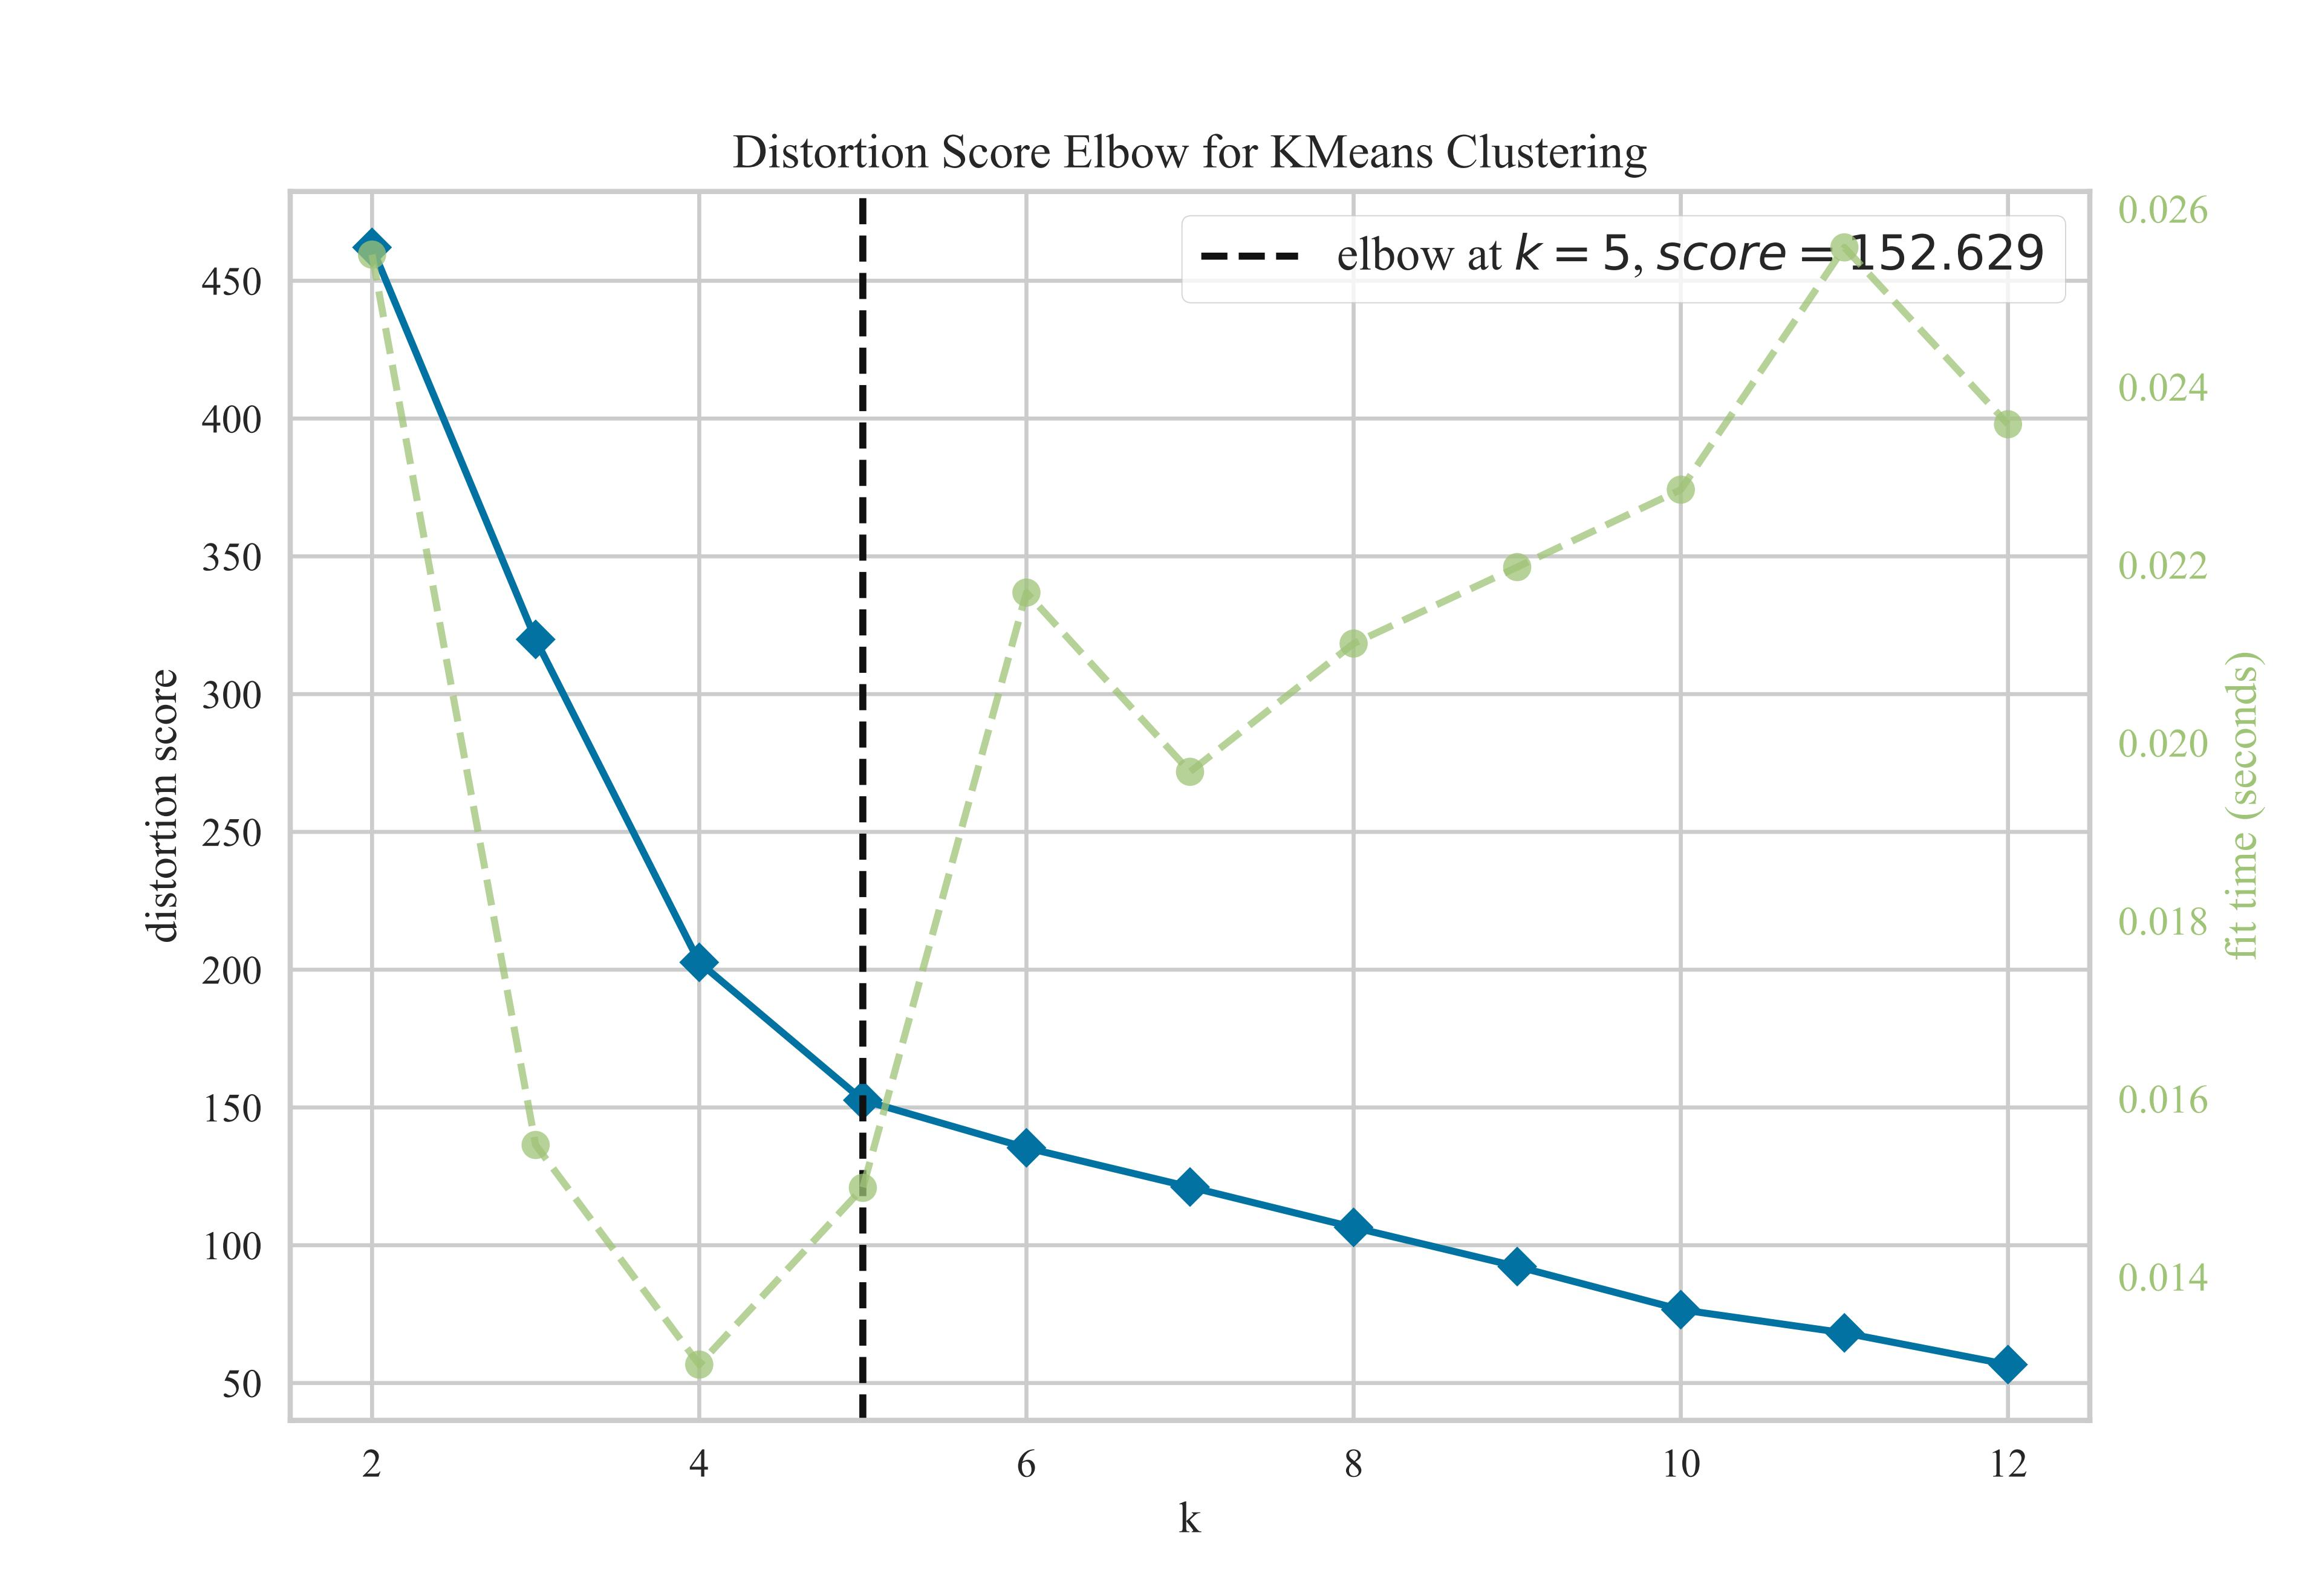
\includegraphics[width=\textwidth]{高钾肘部法则_00.jpg}
			\caption{针对高钾玻璃的肘部法则可视化}%注释1.jpg
			\label{高钾肘部法则}
			\end{minipage}
			\begin{minipage}[t]{0.5\textwidth}
			\centering
			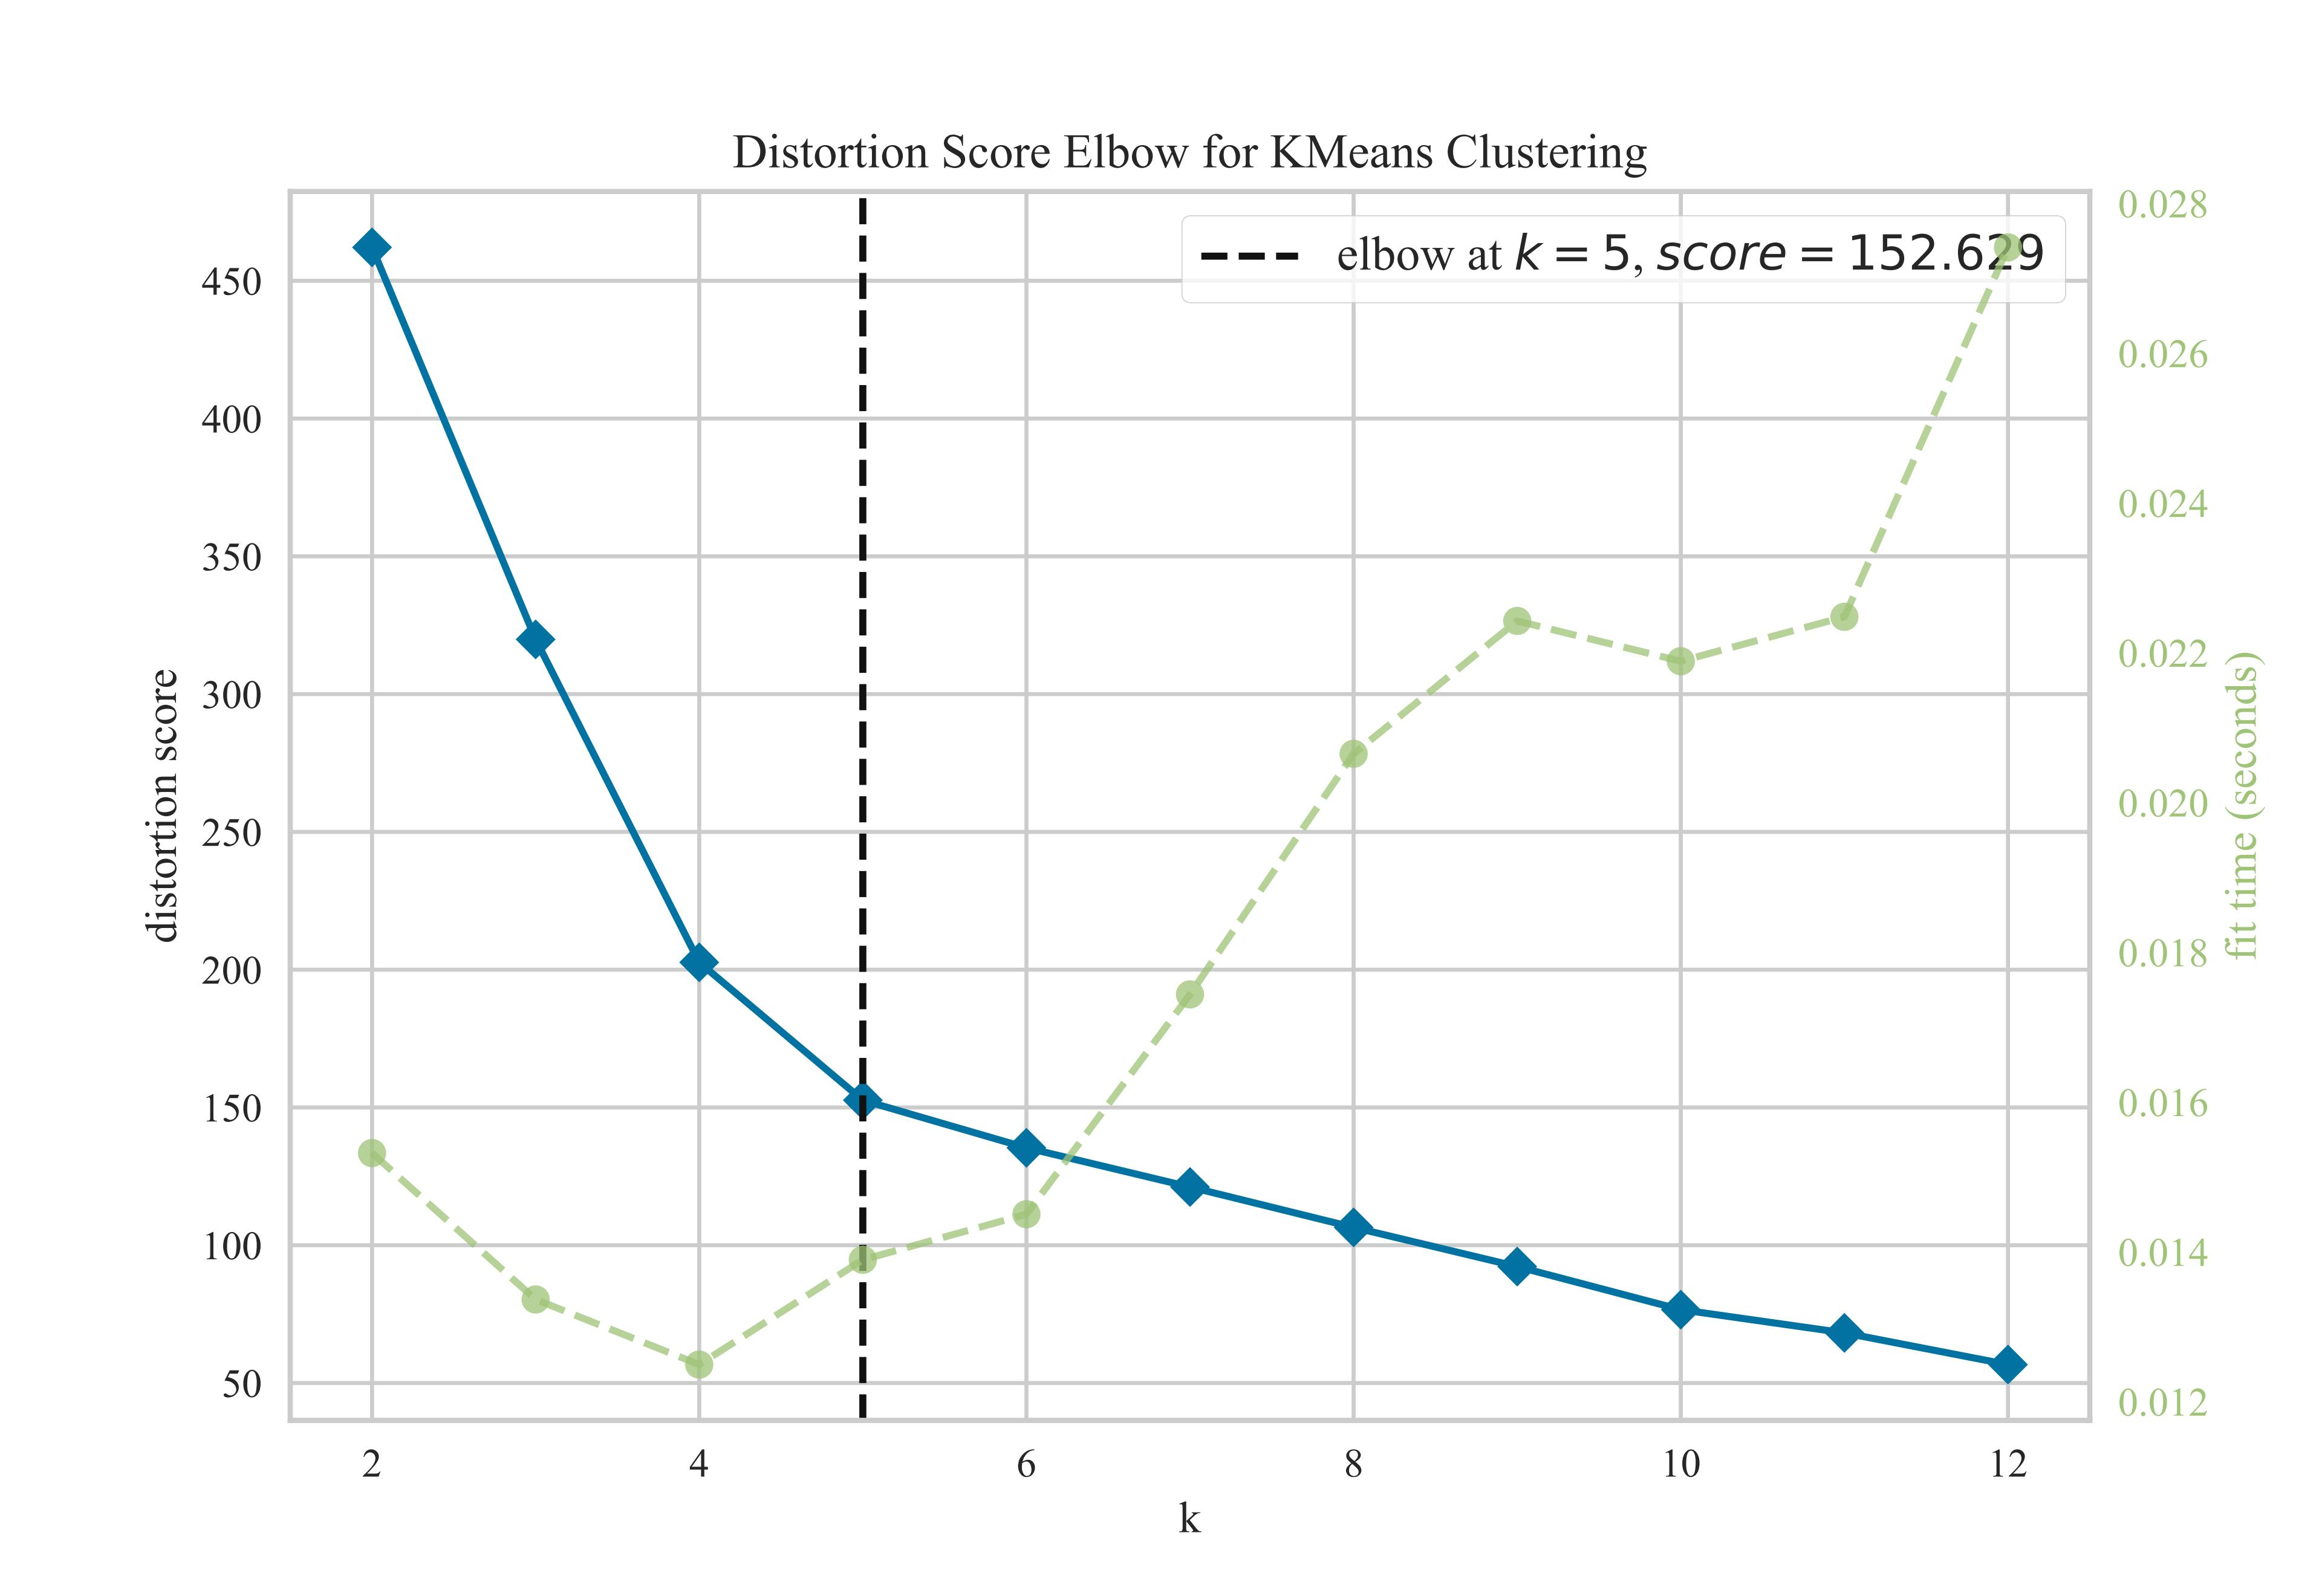
\includegraphics[width=\textwidth]{铅钡肘部法则_00.jpg}
			\caption{针对铅钡玻璃的肘部法则可视化}
			\label{铅钡肘部法则}
			\end{minipage}
		\end{figure}
	
		根据上图,我们可以选择出最适$k$值,即$k$= 5。据此我们对高钾玻璃和铅钡玻璃进行亚类划分,如\textcolor{blue}{\cref{高钾亚类}}和\textcolor{blue}{\cref{铅钡亚类}}所示。
		
% Table generated by Excel2LaTeX from sheet 'Class'
\begin{table}[htbp]
	\centering
	\caption{高钾玻璃亚类划分结果}
	  \begin{tabular}{ccccc}
	  \toprule
	  \textbf{Class} & \multicolumn{4}{c}{\textbf{文物编号}} \\
	  \midrule
	  0     & \multicolumn{4}{c}{1、7、8、9、10、14、16、17} \\
	  1     & \multicolumn{4}{c}{11、12、 13} \\
	  2     & \multicolumn{4}{c}{5} \\
	  3     & \multicolumn{4}{c}{6} \\
	  4     & \multicolumn{4}{c}{0、2、3、4、15} \\
	  \bottomrule
	  \end{tabular}%
	\label{高钾亚类}%
  \end{table}% 
  % Table generated by Excel2LaTeX from sheet 'Class'
  \begin{table}[htbp]
	\centering
	\caption{铅钡玻璃亚类划分结果}
	  \begin{tabular}{cccccccccc}
	  \toprule
	  \textbf{Class} & \multicolumn{9}{c}{\textbf{文物编号}} \\
	  \midrule
	  0     & \multicolumn{9}{c}{3、4、13、14、15、25、28、29、35、38、39、40、43、48} \\
	  1     & \multicolumn{9}{c}{12、30、34} \\
	  2     & \multicolumn{9}{c}{1、2、7、8、9、10、16、17、18、19、20、21、22、23、24、37、41、45、46、47} \\
	  3     & \multicolumn{9}{c}{6、26、27、33} \\
	  4     & \multicolumn{9}{c}{0、5、11、31、32、36、42、44} \\
	  \bottomrule
	  \end{tabular}%
	\label{铅钡亚类}%
  \end{table}%

  \newpage
  \subsection{问题三模型的建立与求解}
  	问题三要求我们分析未知类别玻璃文物的化学成分以确定其所属类别,首先我们分析表单三中的数据是否为有效数据,发现此表单数据均为有效数据。经过综合考虑,我们建立了{\textbf{极端梯度提升(eXtreme Gradient Boosting,XGBoost)模型}},对表单三中的未知文物进行合理的分类。

	XGBoost算法是一种基于树模型的优化模型,该算法通过多次迭代,生成一个新的树模型用于优化前一棵树模型,随着迭代次数的增多,该模型的预测精度也会相应提高\textcolor{blue}{\cite{pxgboost1}}。

	记通过数据处理后的数据集特征为$R\left( x_{ij} \right) _{m\times n}$,表示其包含$m$天的游戏情况,$n$个特征,在训练中形成的CART数的集合记为$F=\left\{ f\left( x \right) =w_{q\left( x \right)},q:\mathbf{R}^n\rightarrow T,w\epsilon \mathbf{R}^T \right\}$,qizhong$q$为树模型的叶节点决策规划,$T$为某一树模型叶节点数量,
	$w$为叶节点对应得分\cite{pxgboost2}。对于预测的$y$值,即$\hat{y}$,计算公式为
	 
	\begin{equation}
		\hat{y}=\varphi \left( x_i \right) =\underset{k=1}{\overset{K}{\Sigma}}f_k\left( x_i \right)
	\end{equation}
	
	XGBoost算法在每一次迭代过程中会保存前面所学习的模型,会将这些模型加入到新一轮迭代过程中,因此我们记第$i$个模型的预测结果为
	
	\begin{equation}
		\hat{y}_{i}^{\left( t \right)}=\hat{y}_{i}^{\left( t-1 \right)}+f_t\left( x_i \right)
	\end{equation}

	XGBoost算法的目标函数计算公式如下
	\begin{equation}
		L^{\left( t \right)}=\underset{i=1}{\overset{n}{\Sigma}}l\left( y_i,\hat{y}_{i}^{\left( t-1 \right)}+f_t\left( x_i \right) \right) +\gamma T+\frac{1}{2}\lambda \underset{j=1}{\overset{T}{\Sigma}}w_{j}^{2}+const
	\end{equation}
	上述公式中,$l$为模型误差损失,描述在该模型下预测值与实际值之间的出差异损失,$\varOmega$为模型叶节点的正则项惩罚系数,$\gamma$和$\lambda$为模型的超参数\textcolor{blue}{\cite{pxgboost2}}。

	通常情况下,我们难以用枚举法得到在模型中所训练出来的树结构,因此这里采用贪婪算法,从单子叶结点开始,通过迭代方法,将其加入到树结构中,从而得到最优解,其计算公式\textcolor{blue}{\cite{pxgboost3}}如下
	\begin{equation}
		\zeta _{split}=\frac{1}{2}\left[ \frac{\left( \Sigma _{i\epsilon I_L}g_i \right) ^2}{\varSigma _{i\epsilon I_L}h_i+\lambda}+\frac{\left( \Sigma _{i\epsilon I_R}g_i \right) ^2}{\Sigma _{i\epsilon I_R}h_i+\lambda}-\frac{\left( \Sigma _{i\epsilon I}g_i \right) ^2}{\Sigma _{i\epsilon I}h_i+\lambda} \right] -\gamma
	\end{equation}
	其中$I_j=\left\{ i|q\left( x_i \right) =j \right\}$为叶节点$j$上的样本集合\textcolor{blue}{\cite{pxgboost2}},且有
	\begin{equation}
		g_i=\partial _{\hat{y}\left( t-1 \right)}l\left( y_i,\hat{y}_{i}^{\left( t-1 \right)} \right) 
	\end{equation}
	\begin{equation}
		h_i=\partial _{\hat{y}\left( t-1 \right)}^{2}l\left( y_i,\hat{y}_{i}^{\left( t-1 \right)} \right) 	
	\end{equation}
	
	\newpage
	依据上述分析,我们{\heiti 首先}以表单三中的文物为分类目标,{\heiti 再}将表单二的数据集按比例7: 3划分为训练集与测试集并通过{\textbf{XGBoost算法}}对训练集和测试集进行训练和评估。 结果如\textcolor{blue}{\cref{分类结果}}所示。
	% Table generated by Excel2LaTeX from sheet '表单3'
\begin{table}[htbp]
	\centering
	\caption{未知玻璃文物分类结果}
	  \begin{tabular}{ccccccccc}
	  \toprule
	  \textbf{文物编号} & A1    & A2    & A3    & A4    & A5    & A6    & A7    & A8 \\
	  \midrule
	  \textbf{类别} & 高钾    & 铅钡    & 铅钡    & 铅钡    & 铅钡    & 高钾    & 高钾    & 铅钡 \\
	  \bottomrule
	  \end{tabular}%
	\label{分类结果}%
  \end{table}%
  
  为检验该模型的敏感性,我们改变了部分文物的部分化学成分比例。调整后的分类结果如\textcolor{blue}{\cref{调整后的分类结果}}所示。
% Table generated by Excel2LaTeX from sheet '表单3'
\begin{table}[htbp]
	\centering
	\caption{调整后未知玻璃文物分类结果}
	  \begin{tabular}{ccccccccc}
	  \toprule
	  \textbf{文物编号} & A1    & A2    & A3    & A4    & A5    & A6    & A7    & A8 \\
	  \midrule
	  \textbf{类别} & 高钾    & 高钾    & 铅钡    & 铅钡    & 铅钡    & 高钾    & 高钾    & 高钾 \\
	  \bottomrule
	  \end{tabular}%
	\label{调整后的分类结果}%
  \end{table}%
 
  由上述调整后的结果可见此模型的敏感性较高,可靠性较高。

  \subsection{问题四模型的建立与求解}
  问题四需要我们针对不同类别的玻璃文物样品,分析化学成分之间的关联关系及不同类别之间的化学成分关联关系的差异性。
  关联关系是指对两个或两个以上存在相关性的因素进行分析,通过计算相关系数并比较,从而判断它们之间的关联程度,得到它们的联系与变化规律。这里我们采用{\textbf{斯皮尔曼相关性分析}}。

  斯皮尔曼相关性分析可以用来评估两个变量相关性的强烈程度,以及它们之间的方向性关系。其原理为考察两个变量的均值和标准偏差,将各自的大小值依次排列,然后计算排列后的值之间的差值($\Delta$),最后依据斯皮尔曼相关系数计算公式算得{\textbf{斯皮尔曼相关系数}}($r$),该系数可以判断两个变量正相关,负相关或无关。
  
  斯皮尔曼相关系数计算公式如下
  \begin{equation}
	r_s=1-\frac{6\underset{i=1}{\overset{n}{\Sigma}}d_{i}^{2}}{n\left( n^2-1 \right)}
  \end{equation}
  其中$d_i$为两组数据之间的等级差。

  \newpage 
  通过上述公式的计算我们得到了相关结果,为了更加直观的展现我们的结果,我们绘制了如\textcolor{blue}{\cref{高钾热力图}}和\textcolor{blue}{\cref{铅钡热力图}}所示的热力图。
  \begin{figure}[htbp]
	\begin{minipage}[t]{0.5\textwidth}%并排放两张图片,每张占页面的0.5,下同。
	\centering
	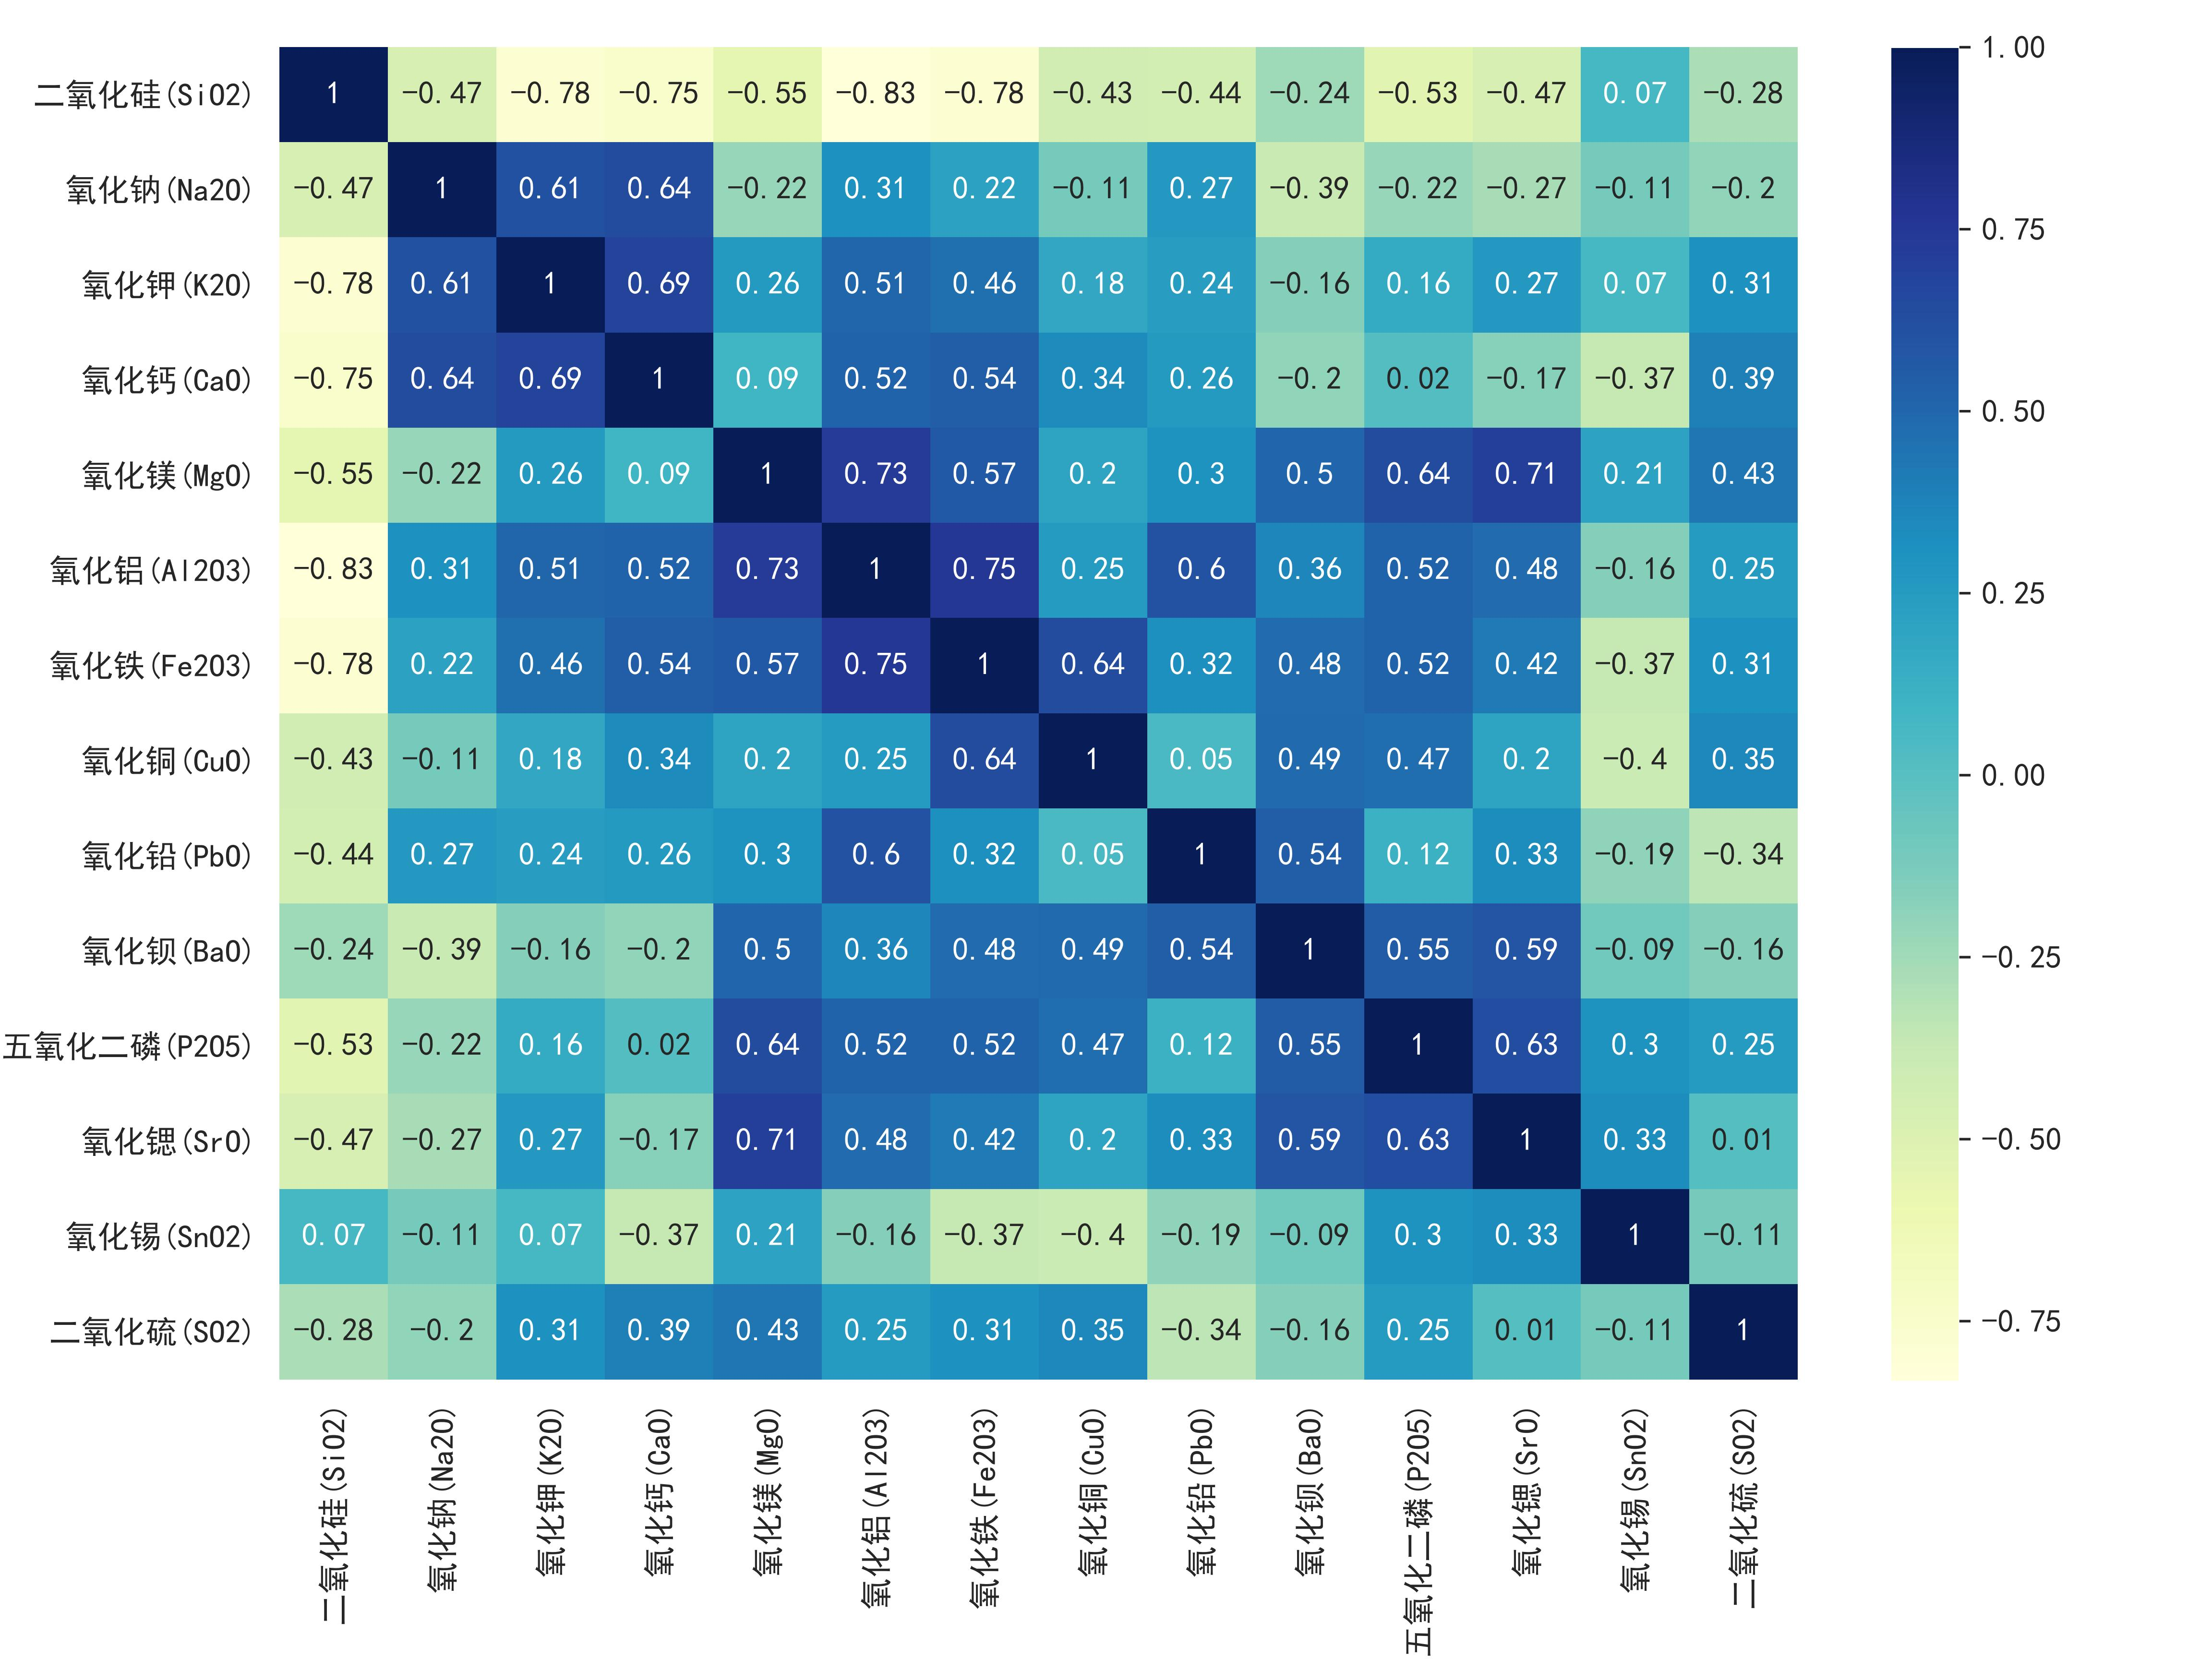
\includegraphics[width=\textwidth]{高钾热力图_00.jpg}
	\caption{高钾玻璃化学成分热力图}%注释1.jpg
	\label{高钾热力图}
	\end{minipage}
	\begin{minipage}[t]{0.5\textwidth}
	\centering
	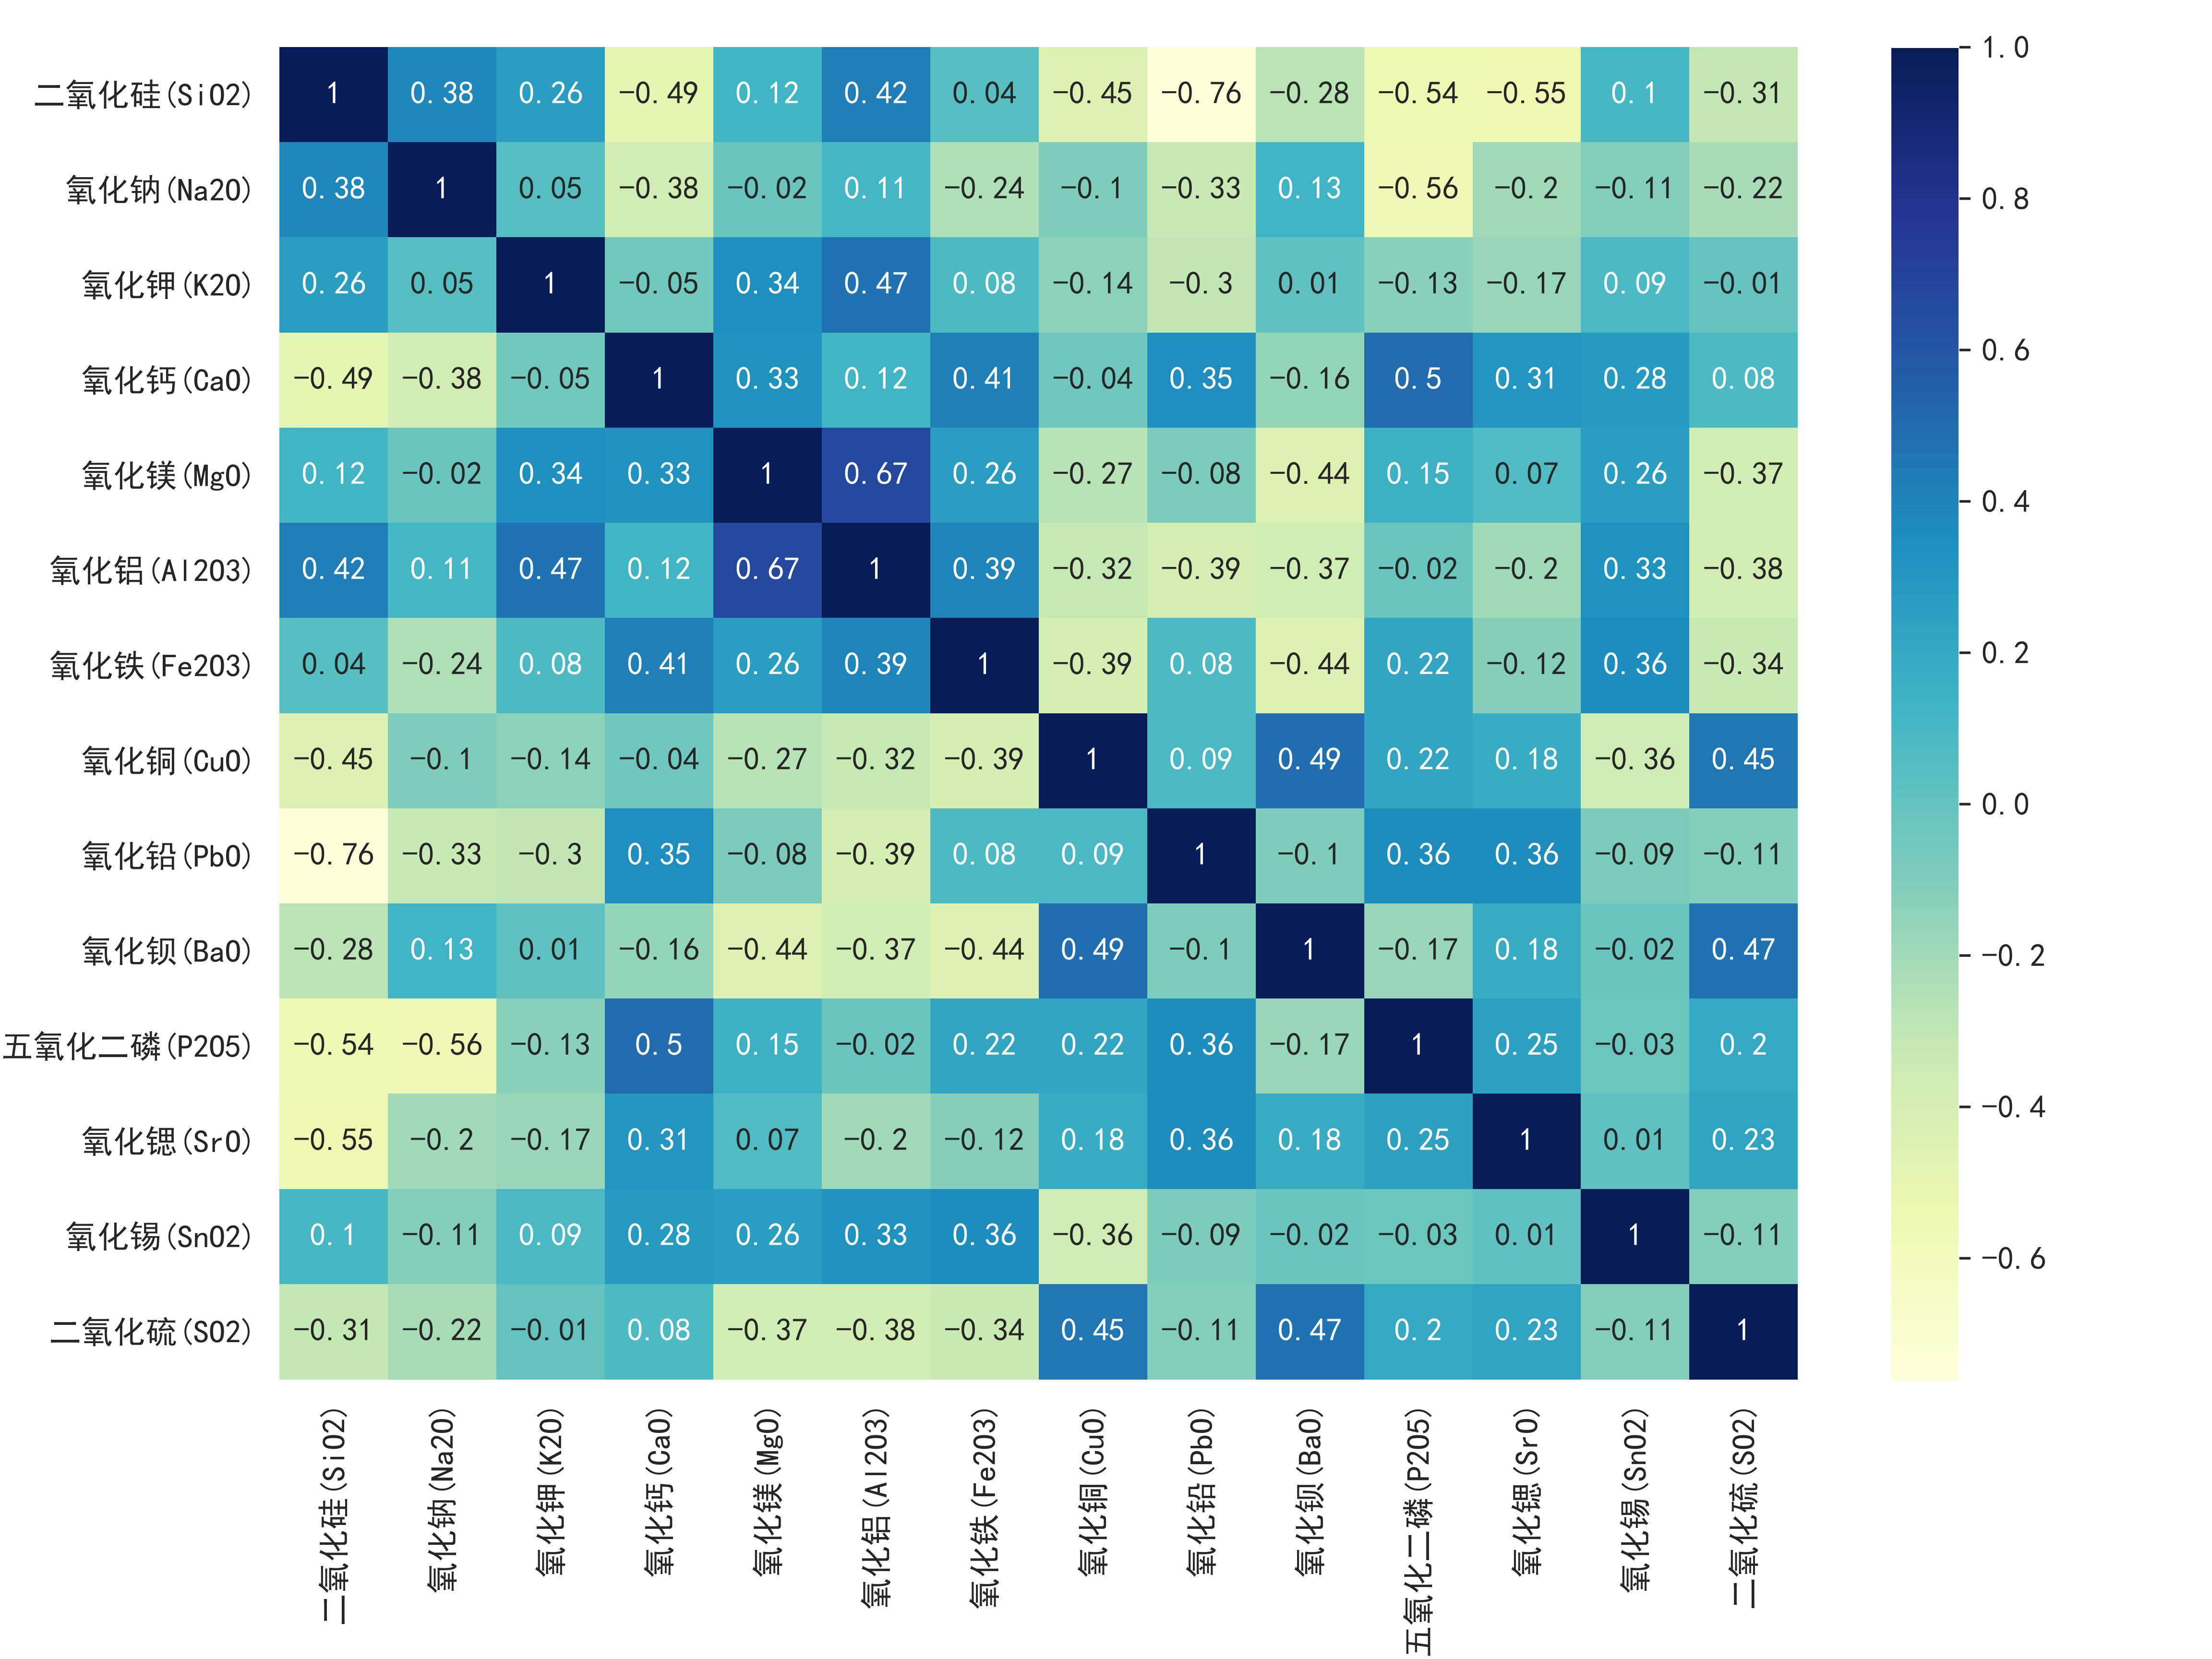
\includegraphics[width=\textwidth]{铅钡热力图_00.jpg}
	\caption{铅钡玻璃化学成分热力图}
	\label{铅钡热力图}
	\end{minipage}
  \end{figure}
  
  我们发现{\textbf{高钾玻璃化学成分热力图}}的色阶图的颜色均较深,我们猜测高钾玻璃各化学成分之间的相关性都较高。其中除主对角线外颜色均较浅,所以高钾玻璃各化学成分之间的关联性都较低。从图中分析可知,高钾玻璃中,两种化学成分呈明显正相关的有氧化镁与氧化铝,呈明显负相关的有二氧化硅与氧化铅。其他成分的相关性较低,可认为其基本没有联系。
  

  对于{\textbf{铅钡玻璃化学成分热力图}},我们发现除主对角线外颜色均较浅,所以铅钡玻璃各化学成分之间的关联性都较低。从图中分析可知,铅钡玻璃中化学成分呈明显正相关的有氧化镁与氧化铝,呈明显负相关的有二氧化硅与氧化铅。其他成分的相关性较低,可认为其基本没有联系。

  对于{\heiti 不同类别之间的化学成分关联关系的差异性},我们通过对比高钾玻璃和铅钡玻璃的热力图,颜色差异较大处对应的两个化学成分斯皮尔曼相关系数数值上相差较大,即两种玻璃关于这两种化学成分的相关性差异较大。由于涉及化学成分较多,此处选取一组具有{\heiti 明显差异性}的化学成分进行分析作为示例:两种玻璃
  中{\textbf{二氧化硅和氧化铝}}的相关性虽然接近,但在铅钡玻璃中两者为正相关性,而在高钾玻璃中两者为负相关性。

\newpage
\section{模型的评价与推广}
\subsection{模型的评价}
\begin{itemize}
	\item \textbf{模型的优点}:
	
	1.对数据进行预处理时,我们{\textbf{以0.04而非0}}填充空缺值,数据的误差更小且更真实。
	
	2.利用K-means聚类,结合肘部法则,选择最优聚类k值,聚类结果更精确。
	
	3.可视化分析问题,结果直观易理解。
	
	4.对玻璃进行聚类之后与题目的文字叙述进行对比,验证了结果的合理性。
	
	\item \textbf{模型的缺点}:
	
	1.在研究定类变量的关系时,由于数据较少,卡方检验的误差增大,当存在很大误差时,可使用Fisher精确检验代替卡方检验。
	
	2.数据量偏少,可能会影响模型的准确程度,易出现“过拟合”现象

	3.对于分类的结果未采用其他模型进行验证。

\end{itemize}

\subsection{模型的推广}
XGboost 聚类预测模型可较好地对事物进行分类并预测未知的类别,因此其有利于对已知未分类事物进行分类,并分析预测出新事物的类别。我们认为该模型可应用于物种鉴定等领域。总而言之,本文所建立模型有着泛化能力较强、精度较高的优秀品质,可为医疗,生物,考古等多行业提供有利帮助。
	
\newpage
	\phantomsection
	\addcontentsline{toc}{section}{\textbf{参考文献}}
	\begin{spacing}{1.08}
	\begin{thebibliography}{99}
	\bibitem{pxgboost1}陈振宇,刘金波,李晨,季晓慧,李大鹏,黄运豪,狄方春,高兴宇,徐立中.基于LSTM与XGBoost组合模型的超短期电力负荷预测[J].电网技术,2020,44(02):614-620.DOI:10.13335/j.1000-3673.pst.2019.1566.

	\bibitem{pxgboost2}杨贵军,徐雪,赵富强.基于XGBoost算法的用户评分预测模型及应用[J].数据分析与知识发现,2019,3(01):118-126.

	\bibitem{pxgboost3}Tianqi Chen and Carlos Guestrin. 2016. XGBoost: A Scalable Tree Boosting System. In Proceedings of the 22nd ACM SIGKDD International Conference on Knowledge Discovery and Data Mining (KDD '16). Association for Computing Machinery, New York, NY, USA, 785–794. \url{https://doi.org/10.1145/2939672.2939785}.

	\bibitem{ppearson1}肖杨,李亚,王海瑞,常梦容.基于皮尔逊相关系数的滚动轴承混合域特征选择方法[J].化工自动化及仪表,2022,49(03):308-315.DOI:10.20030/j.cnki.1000-3932.202203009.
	
	\bibitem{ppearson2}王殿武,赵云斌,尚丽英,王凤刚,张震.皮尔逊相关系数算法在B油田优选化学防砂措施井的应用[J].精细与专用化学品,2022,30(07):26-28.DOI:10.19482/j.cn11-3237.2022.07.07.

	\bibitem{psvm}汪海燕,黎建辉,杨风雷.支持向量机理论及算法研究综述[J].计算机应用研究,2014,31(05):1281-1286.

	\bibitem{卡方检验}百度百科【卡方检验】[EO/BL].\url{https://baike.baidu.com/item/%E5%8D%A1%E6%96%B9%E6%A3%80%E9%AA%8C/2591853}.

	\bibitem{卡方检验2}百家号【如何简单理解卡方检验?】[EO/BL].\url{https://baijiahao.baidu.com/s?id=1771127457087657402&wfr=spider&for=pc}.

	\bibitem{斯皮尔曼相关性}百度百科【斯皮尔曼相关性分析】[EO/BL].\url{https://wenku.baidu.com/view/f4e06f5975c66137ee06eff9aef8941ea76e4b38.html?_wkts_=1690549232319&bdQuery=%E6%96%AF%E7%9A%AE%E5%B0%94%E6%9B%BC%E7%9B%B8%E5%85%B3%E6%80%A7%E5%88%86%E6%9E%90%E5%8E%9F%E7%90%86}

	\end{thebibliography}
	\end{spacing}
	\newpage

	\phantomsection
	\addcontentsline{toc}{section}{\textbf{附\hspace{2pc}录}}

	% \appendix
	% \ctexset{section={format={\zihao{-4}\heiti\raggedright}}}
	\begin{center}
		\heiti\zihao{4} 附\hspace{2pc}录
	\end{center}

% \phantomsection
% \addcontentsline{toc}{subsection}{[A]图示}
	% \section*{[A]图示}
	\noindent{\heiti [A]图示}
	\begin{figure}[H]
		\centering
		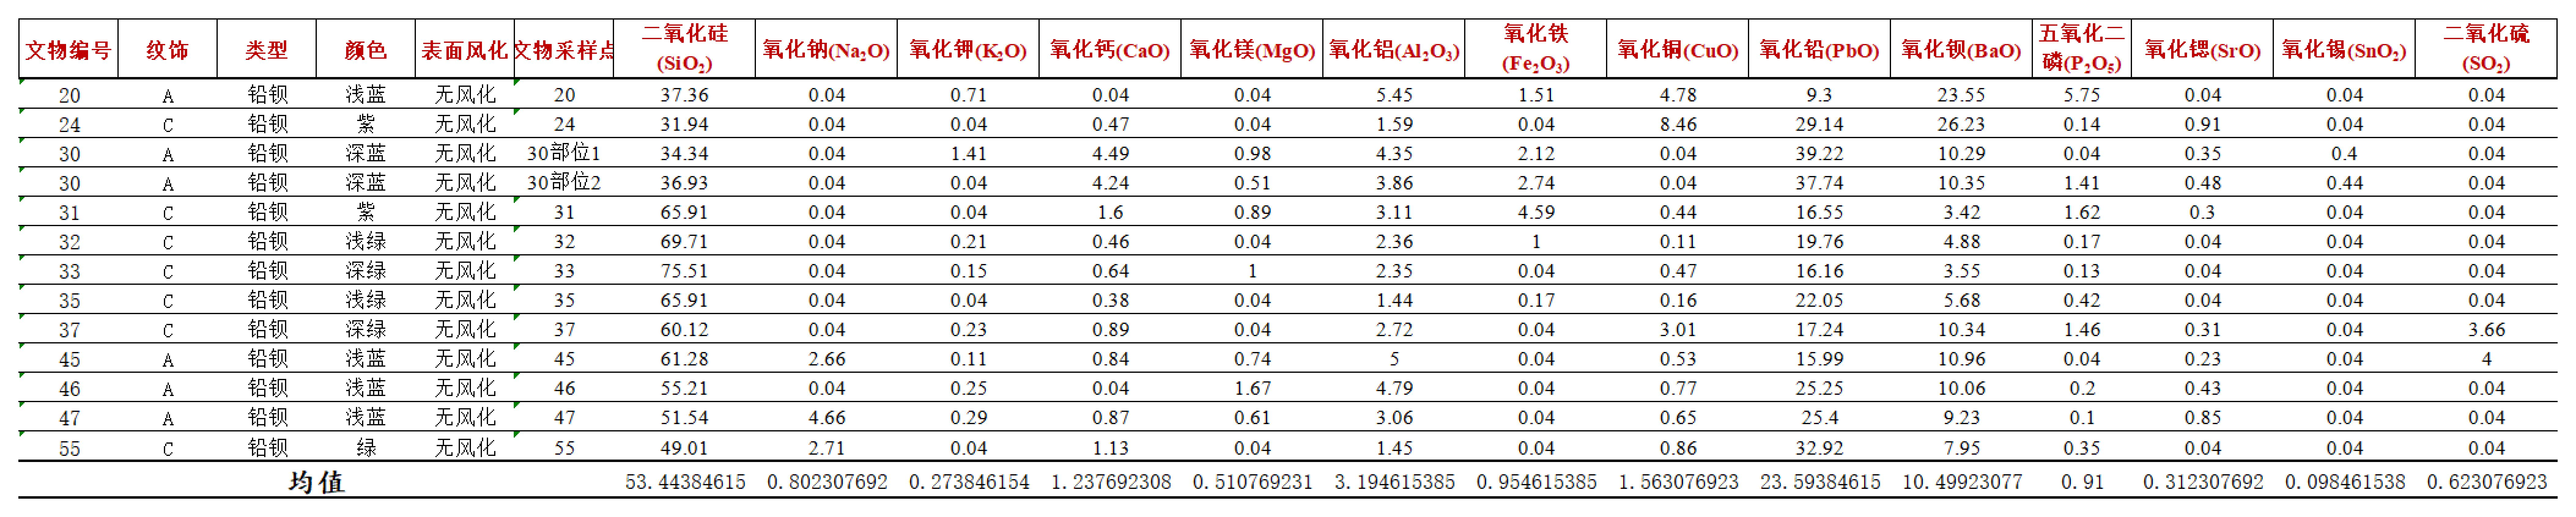
\includegraphics[width=1.0\textwidth]{铅钡第一问第二小问_00.jpg}
		\caption{铅钡玻璃未风化相关数据}
		\label{铅钡未风化}
	\end{figure}
	\begin{figure}[H]
		\centering
		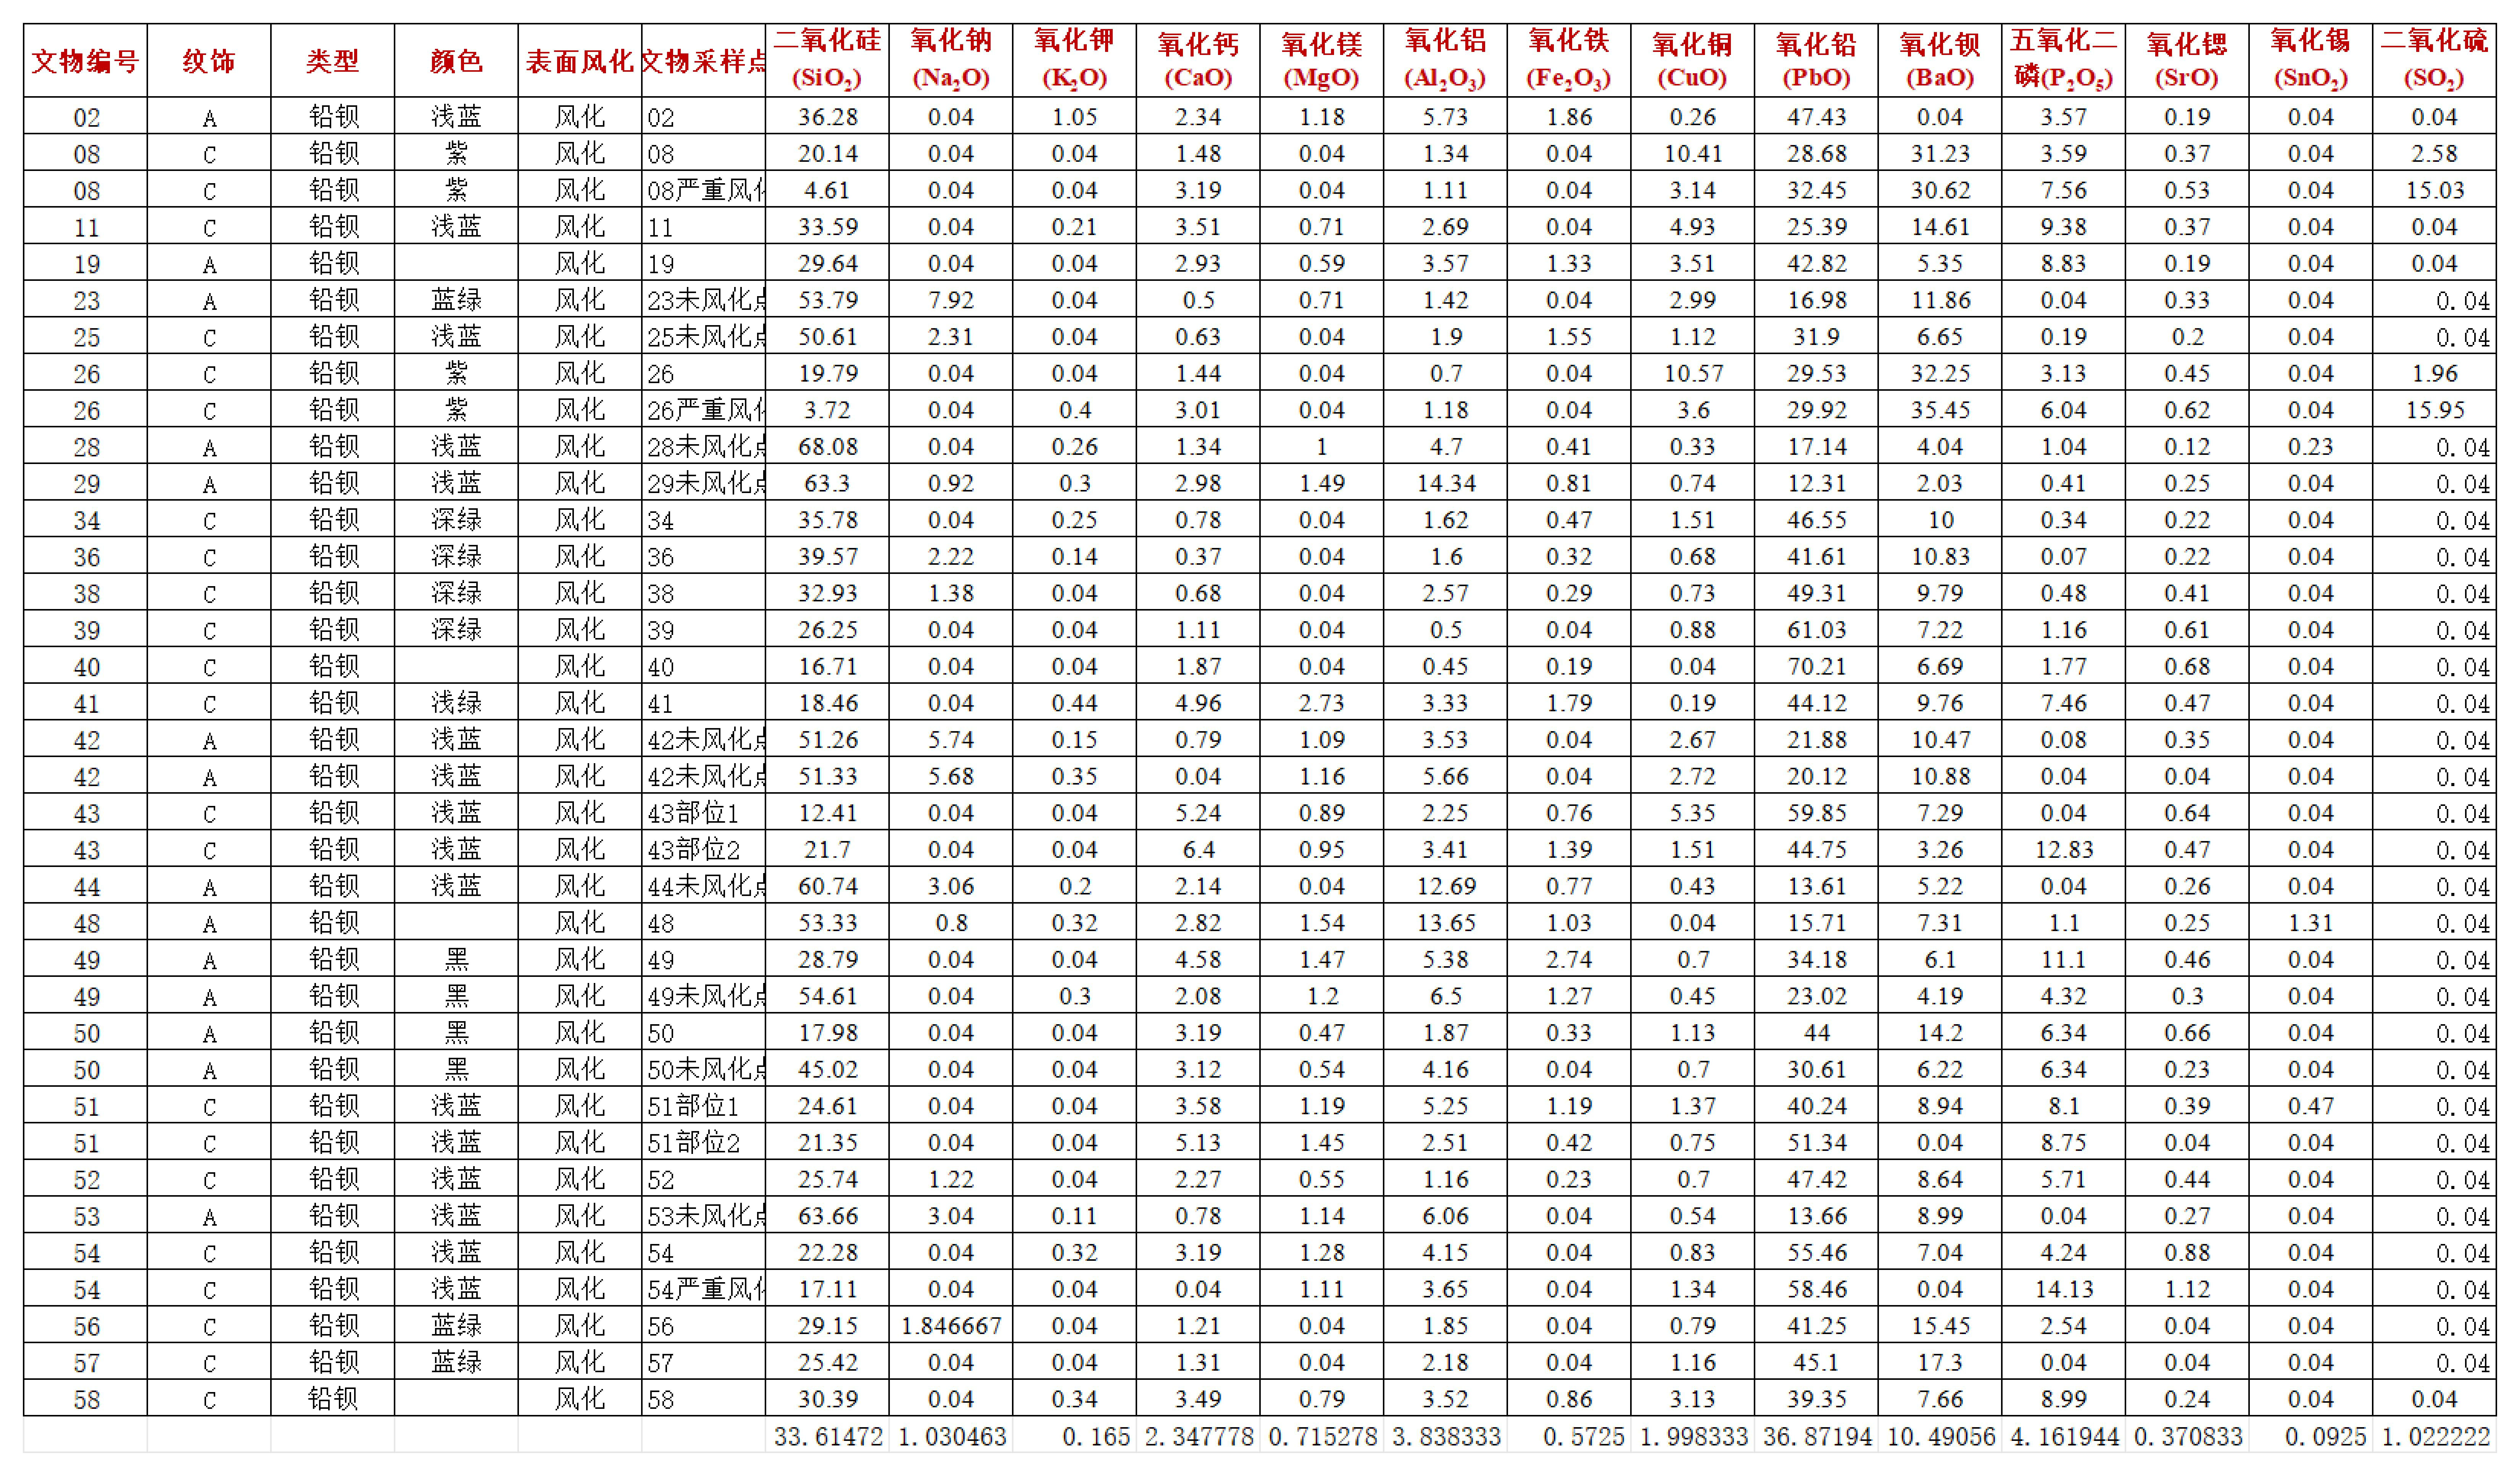
\includegraphics[width=1.0\textwidth]{铅钡第一问第二小问_01.jpg}
		\caption{铅钡玻璃风化相关数据}
		\label{铅钡风化}
	\end{figure}
	\begin{figure}[H]
		\centering
		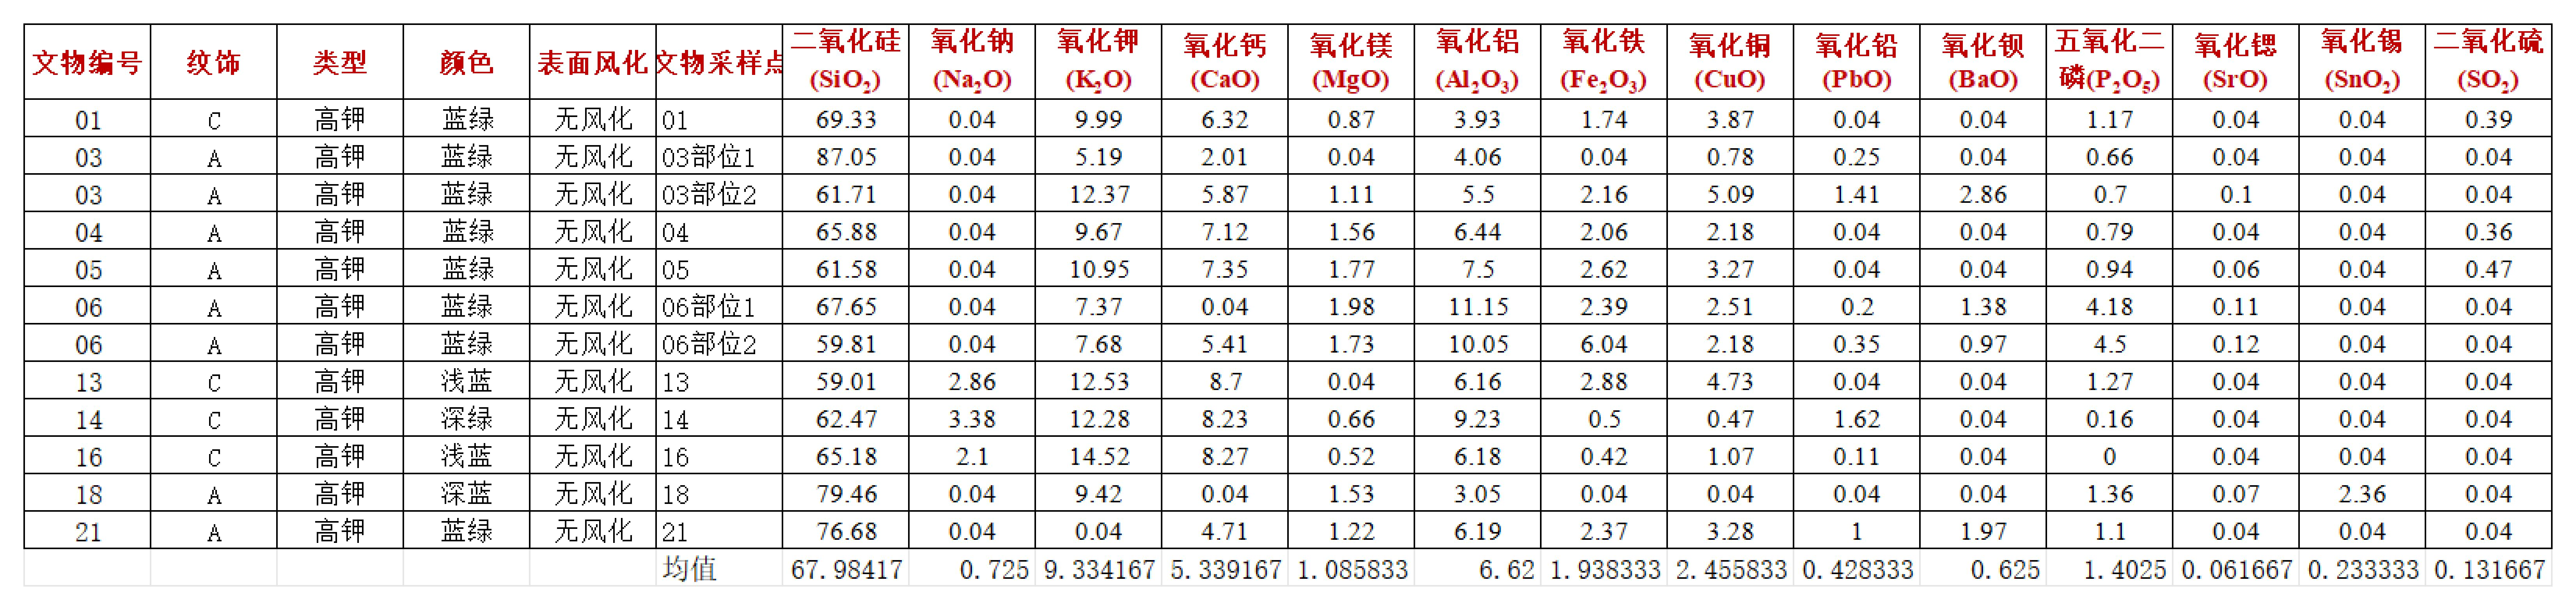
\includegraphics[width=1.0\textwidth]{高钾第一问第二小问_00.jpg}
		\caption{高钾玻璃未风化相关数据}
		\label{高钾未风化}
	\end{figure}
	\begin{figure}[H]
		\centering
		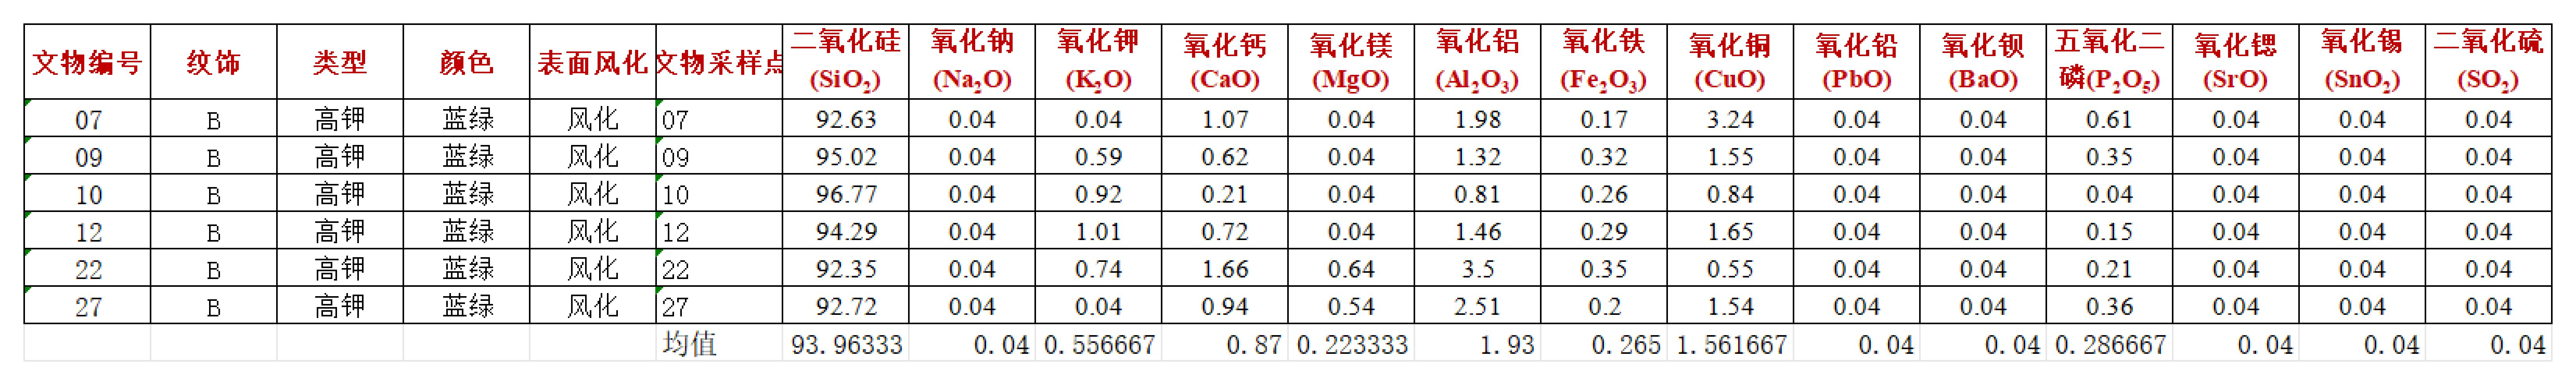
\includegraphics[width=1.0\textwidth]{高钾第一问第二小问_01.jpg}
		\caption{高钾玻璃风化相关数据}
		\label{高钾风化}
	\end{figure}	
	
	\newpage
	\noindent{\heiti [B]支撑文件列表}
	~\\

	支撑文件列表如下(按文件夹进行分类):

\begin{table}[H]   
	\centering     
	\begin{tabular}{cc}     
		\toprule     
		\textbf{文件夹名} & \textbf{描述} \\     
		\midrule     
		Code  & 解决问题所有源程序,包括ipynb及其对应的py文件 \\     Figures & 论文中所有矢量图示,均为pdf文件 \\     
		Data  & 解决问题所用数据,均为xlsx文件 \\     
		Result & 程序输出结果,均为html文件 \\     
		\bottomrule     
	\end{tabular}
\end{table}

\newpage
	\noindent{\heiti [C]使用的软件、环境}
	~\\

	\textbf{C.1}:为解决该问题,我们所使用的主要软件有:
	\begin{itemize}
		\item TeX Live 2022
		\item Visual Studio Code 1.77.3
		\item WPS Office 2023春季更新(14036)
		\item Python 3.10.4
		\item Pycharm 2023.1.1 (Professional Edition)
	\end{itemize}

	\textbf{C.2}:Python环境下所用使用到的库及其版本如下:
\begin{table}[H]
	\centering
	\setlength{\aboverulesep}{0pt}
	\setlength{\belowrulesep}{0pt}
	\scalebox{0.90}{
	  \begin{tabular}{cc||cc}
	  \toprule
	  \textbf{库} & \textbf{版本} & \textbf{库} & \textbf{版本} \\
	  \midrule
	  copy  & 内置库   & matplotlib & 3.5.2 \\
	  jupyter & 1.0.0 & nltk  & 3.7 \\
	  jupyter-client & 7.3.1 & numpy & 1.22.4+mkl \\
	  jupyter-console & 6.4.3 & openpyxl & 3.0.10 \\
	  jupyter-contrib-core & 0.4.0 & pandas & 1.4.2 \\
	  jupyter-contrib-nbextensions & 0.5.1 & scikit-learn & 0.22.2 psot1 \\
	  jupyter-highlight-selected-word & 0.2.0 & seaborn & 0.11.2 \\
	  jupyterlab-pygments & 0.2.2 & sklearn & 0 \\
	  jupyterlab-widgets & 1.1.0 & xgboost & 1.6.1 \\
	  jupyter-latex-envs & 1.4.6 & yellowbrick & 1.4 \\
	  jupyter-nbextensions-configurator & 0.5.0 &       &  \\
	  \bottomrule
	  \end{tabular}}
\end{table}
  
\newpage

\noindent{\heiti [D]问题解决源程序}



\end{document}